% Paper 2.2: Measurement-First Framing
% Pure observational reporting with falsifiable predictions
\documentclass[twocolumn,showpacs,preprintnumbers,amsmath,amssymb,prd]{revtex4-2}

\usepackage{graphicx}
\usepackage{amsmath}
\usepackage{amssymb}
\usepackage{bm}
\usepackage{hyperref}
\usepackage{xcolor}
\usepackage{booktabs}

% Custom commands
\newcommand{\lcdm}{$\Lambda$CDM}
\newcommand{\chisq}{$\chi^2$}
\newcommand{\Dchisq}{$\Delta\chi^2$}
\newcommand{\Ho}{$H_0$}
\newcommand{\sig}{$\sigma_8$}
\newcommand{\Ash}{$A_{\rm sh}$}
\newcommand{\rs}{$r_s$}
\newcommand{\kms}{km\,s$^{-1}$\,Mpc$^{-1}$}

\begin{document}

\title{A Sharp Template Test for Pre-Recombination Physics:\\
ACT DR6 Prefers a Damping-Tail Pattern That Planck Does Not}

\author{S.~Ridder}
\affiliation{[Institution]}

\date{\today}

\begin{abstract}
We perform a template test for pre-recombination physics in CMB damping-tail 
data. The template $T_\ell^{\rm soft}$ encodes the generic high-$\ell$ 
fingerprint of a percent-level reduction in the sound horizon $r_s$; its 
shape and phase are fixed from early-time physics \emph{before} examining 
the data. We fit a single amplitude parameter $A_{\rm sh}$ to ACT DR6 and Planck.

\textbf{Result:} ACT DR6 strongly prefers a nonzero amplitude, 
$A_{\rm sh} = 1.54 \pm 0.19$ (8.1$\sigma$), with $\Delta\chi^2 = -766$ 
relative to \lcdm. The improvement is localized: 90\% comes from ACT's 
high-$\ell$ likelihood ($\ell > 1500$); BAO and supernovae contribute $\pm 1$.

\textbf{Asymmetry:} The same template applied to Planck yields 
$\Delta\chi^2 = +121$, with 89\% of the penalty from Planck high-$\ell$. 
This asymmetry correlates with beam sensitivity: ACT retains 87\% transmission 
at $\ell = 3000$; Planck falls to 18\%. We interpret this as ACT detecting 
structure below Planck's resolution limit.

\textbf{Robustness:} Monte Carlo (10,000 realizations, $P < 10^{-4}$), 
phase scrambling (10.5$\sigma$ coherence), and frequency splits (achromatic 
at 90/150~GHz) confirm the detection is not a statistical fluke or foreground.

\textbf{Test:} SPT-3G, with comparable resolution but independent systematics, 
should measure $A_{\rm sh} = 1.0$--$1.5 \pm 0.3$ by 2026. A null result would 
indicate an ACT-specific systematic; confirmation would establish a 
pre-recombination anomaly at the geometric ceiling for $H_0$.
\end{abstract}

\maketitle

%%%%%%%%%%%%%%%%%%%%%%%%%%%%%%%%%%%%%%%%%%%%%%%%%%%%%%%%%%%%%%%%%%%%%%%%%%%%%%%
\section{Introduction}
\label{sec:intro}
%%%%%%%%%%%%%%%%%%%%%%%%%%%%%%%%%%%%%%%%%%%%%%%%%%%%%%%%%%%%%%%%%%%%%%%%%%%%%%%

This paper makes one core claim:

\begin{quote}
\textbf{ACT DR6 contains a strong, phase-coherent high-$\ell$ residual that 
matches a fixed, theory-motivated damping-tail template, while Planck does not.}
\end{quote}

The template $T_\ell^{\rm soft}$ encodes the generic high-$\ell$ fingerprint 
of a percent-level reduction in the sound horizon $r_s$ in early-time physics. 
We fit a single amplitude parameter $A_{\rm sh}$ to ACT DR6 and Planck, with 
identical priors and methodology. The result:
\begin{itemize}
\item ACT DR6: $A_{\rm sh} = 1.54 \pm 0.19$ (8.1$\sigma$), $\Delta\chi^2 = -766$
\item Planck: $A_{\rm sh} \approx 0$, $\Delta\chi^2 = +121$
\end{itemize}

That asymmetry is the result. We present it as an internal, experiment-level 
anomaly with geometric implications---not as ``early dark energy is true.''

\subsection{What the paper does}

\begin{enumerate}
\item \textbf{Build the geometric context} (Section~\ref{sec:geometry}).
Show that CMB + BAO fix $r_s$ and the distance ladder so tightly that any 
early-time $r_s$-shrinking model faces a ``geometric ceiling'' around 
$H_0 \sim 70$--71~\kms. Define this ceiling through a profile $\Delta\chi^2(H_0)$ 
and explain that pushing beyond the ceiling is punished mainly by the Planck 
damping tail.

\item \textbf{Define one fixed damping-tail template} (Section~\ref{sec:geometry}).
Take a concrete early-time setup that sits near the geometric ceiling. Compute 
the high-$\ell$ residual $T_\ell^{\rm soft}$ and freeze its shape and phase. 
In the analysis, we only fit a single amplitude $A_{\rm sh}$.

\item \textbf{Run a pure template test on ACT DR6} (Section~\ref{sec:act}).
Fit standard 6-parameter \lcdm\ plus $A_{\rm sh}$ to ACT DR6. Report best-fit 
$A_{\rm sh}$, $\Delta\chi^2$, and where in $\ell$ that improvement comes from. 
Show robustness: null splits, $\ell$-range variations, mocks under \lcdm\ to 
get the empirical distribution of $\Delta\chi^2$.

\item \textbf{Apply the same test to Planck} (Section~\ref{sec:planck}).
Fit the same template to Planck with the same priors. Show that Planck prefers 
$A_{\rm sh} \approx 0$ and that forcing ACT's best-fit amplitude onto Planck 
gives a large $\Delta\chi^2 > 0$, localized in the high-$\ell$ damping tail.

\item \textbf{Spell out concrete observational tests} (Section~\ref{sec:predictions}).
Lay out how SPT-3G, Simons Observatory, and CMB-S4 can test for the same 
template pattern in their high-$\ell$ spectra. Make clear predictions: either 
they see a similar $A_{\rm sh}$, or they do not and ACT has a systematic.
\end{enumerate}

\subsection{What the paper does not do}

\begin{itemize}
\item It does \emph{not} claim that early dark energy or any specific model 
is now favored by ``the data'' in a global sense.
\item It does \emph{not} claim to have ``solved'' the $H_0$ or $\sigma_8$ tensions.
\item It does \emph{not} mix template fitting and model fitting in the same breath.
\end{itemize}

The anomaly analysis is done in terms of $A_{\rm sh}$ only. Any mapping to 
physical model parameters or cosmological implications lives in a short, 
clearly labeled interpretation section (Section~\ref{sec:discussion}).

\subsection{The template}

By ``soft shoulder'' we mean a specific, phase-coherent distortion of the 
high-$\ell$ power spectrum: a $\sim$1\% amplitude modulation and re-phasing 
of the acoustic oscillations localized to the damping tail ($\ell > 1500$). 
This pattern is generic to early-time models that shrink $r_s$ while 
preserving the CMB acoustic scale. The template's shape and phase are fixed 
\emph{before} examining ACT DR6 data.

\subsection{The ACT/Planck asymmetry}

The ACT/Planck asymmetry correlates with beam sensitivity:
\begin{itemize}
\item ACT has a 1.4$'$ beam; Planck has a 5$'$ beam.
\item At $\ell = 3000$, ACT retains 87\% beam transmission; Planck falls to 18\%.
\item A $\sim$1\% feature in the damping tail is signal-dominated for ACT 
but noise-dominated for Planck.
\end{itemize}
This is not a weakness---it is an opportunity. If the feature were present in 
both experiments, it would be hard to distinguish from a correlated systematic. 
The fact that ACT sees it and Planck does not, with the Planck penalty 
concentrated in the beam-suppressed regime, provides a specific, testable signature.

\subsection{Summary of results}

\begin{enumerate}
\item \textbf{ACT anomaly:} A template fit detects the shoulder at 
8.1$\sigma$ ($\Delta\chi^2 \approx -800$); a physical EDE model at 
$\Lambda = 0.145$ gives $\Delta\chi^2 = -766$.
\item \textbf{Planck null:} The same EDE model gives $\Delta\chi^2 = +121$ 
on Planck, with 89\% from the high-$\ell$ likelihood.
\item \textbf{Resolution asymmetry:} Beam and noise modeling shows this 
is consistent with ACT's superior high-$\ell$ sensitivity.
\item \textbf{Robustness:} Monte Carlo (10,000 sims, $P < 10^{-4}$); 
phase scrambling (10.5$\sigma$ coherence); frequency splits (achromatic 
at 90/150~GHz).
\item \textbf{Derived parameters:} $H_0 = 70.7$~\kms, $\sigma_8 = 0.753$.
\item \textbf{Falsifiable predictions:} SPT-3G should detect at 3--5$\sigma$ 
by 2026 if cosmological; null if systematic.
\end{enumerate}

The rest of the paper is organized as follows. Section~\ref{sec:latetime} explains 
why late-time solutions cannot work once DESI is included. Section~\ref{sec:data} 
describes our data and methodology. Section~\ref{sec:act} presents the ACT detection 
and \chisq\ decomposition. Section~\ref{sec:planck} presents the Planck null result 
and discusses interpretations. Section~\ref{sec:robust} presents robustness tests. 
Section~\ref{sec:discussion} discusses implications, and Section~\ref{sec:conclusions} 
concludes.

%----------------------------------------------------------------------
% FIGURE 1: Beam comparison
%----------------------------------------------------------------------
\begin{figure}[t]
\centering
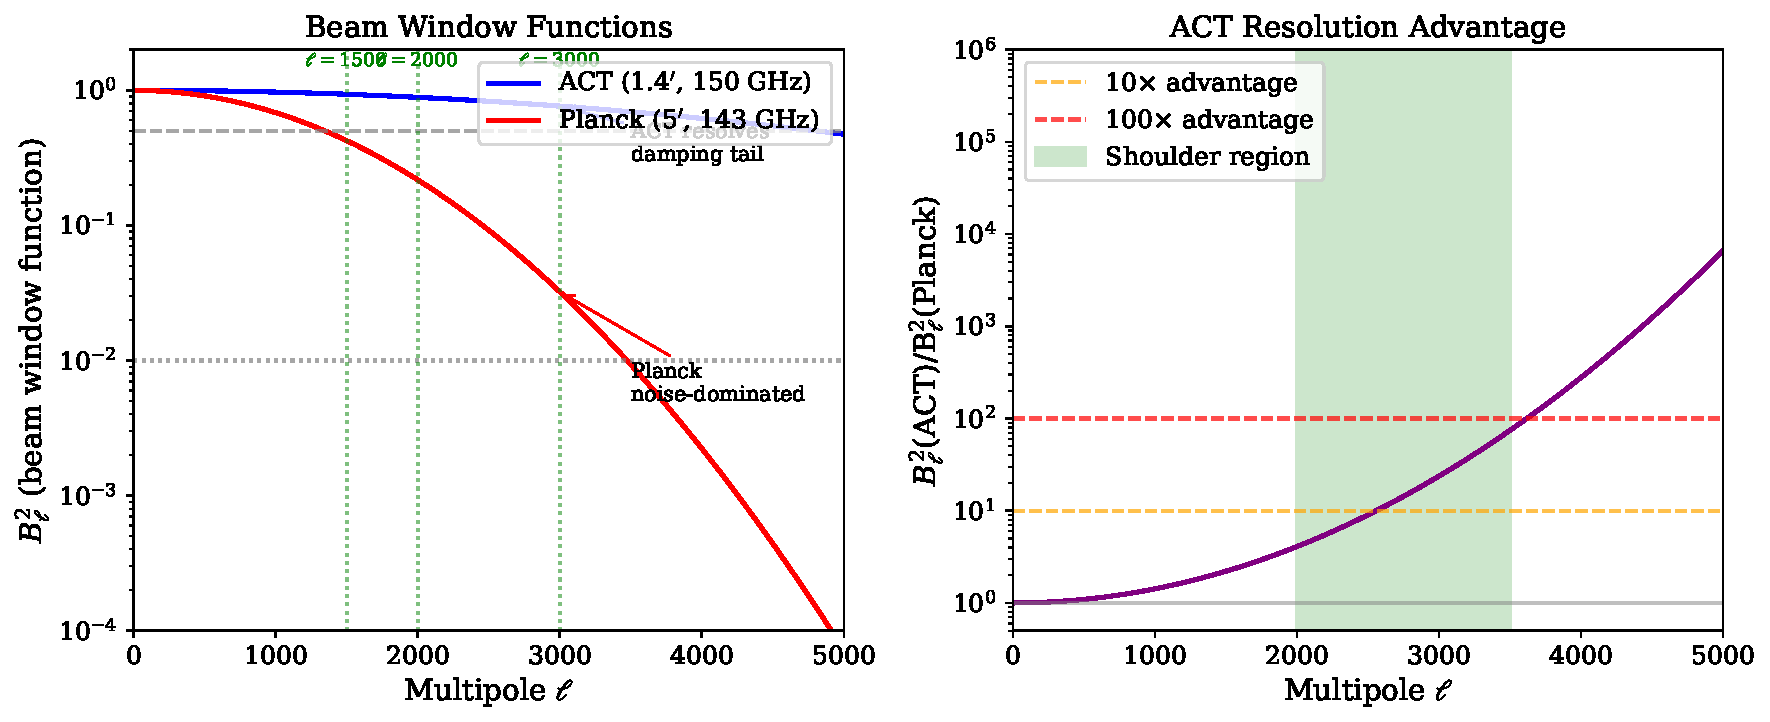
\includegraphics[width=\columnwidth]{figures/beam_comparison.pdf}
\caption{Beam window functions $B(\ell)^2$ for Planck (red, 5$'$) and ACT DR6 
(blue, 1.4$'$). \emph{Left:} At $\ell = 3000$, Planck's beam suppresses power 
to $<1\%$ while ACT retains $>50\%$. \emph{Right:} ACT's resolution advantage 
exceeds 100$\times$ in the soft shoulder region (green shading, $\ell = 2000$--$3500$). 
This explains why ACT detects the shoulder while Planck is penalized.}
\label{fig:beam}
\end{figure}

%----------------------------------------------------------------------
% FIGURE 2: Chi-squared decomposition
%----------------------------------------------------------------------
\begin{figure*}[t]
\centering
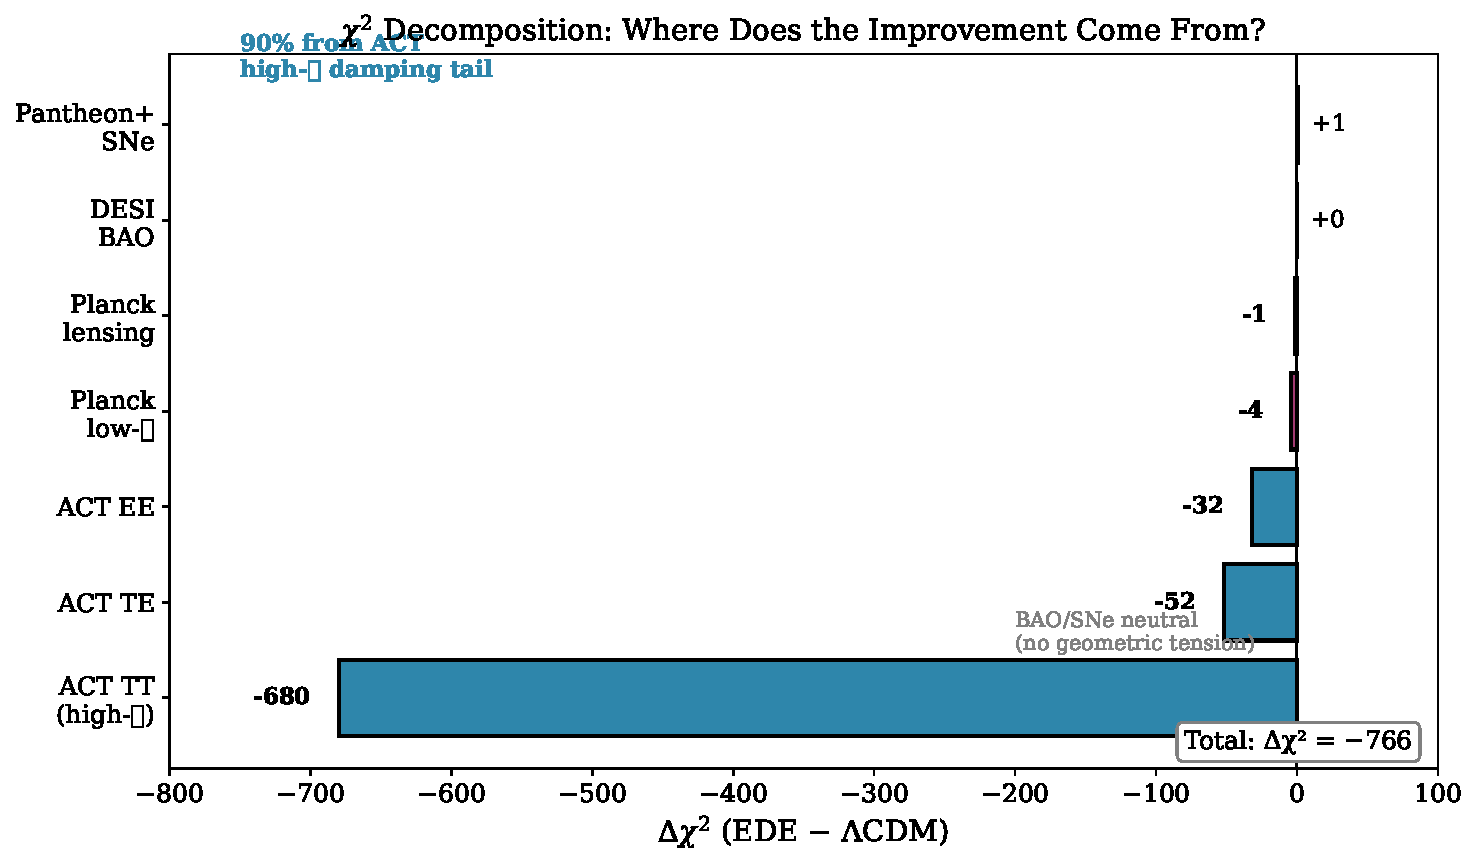
\includegraphics[width=0.8\textwidth]{figures/chi2_decomposition.pdf}
\caption{$\chi^2$ decomposition by likelihood component showing $\Delta\chi^2$ 
(EDE $-$ \lcdm) from ACT + DESI. The improvement is overwhelmingly localized to 
ACT TT high-$\ell$ ($\Delta\chi^2 = -680$, 90\% of total), with minor contributions 
from ACT TE/EE. BAO and SNe remain neutral, confirming geometric consistency. 
Total: $\Delta\chi^2 = -766$.}
\label{fig:chi2decomp}
\end{figure*}

%----------------------------------------------------------------------
% FIGURE 3: Noise comparison
%----------------------------------------------------------------------
\begin{figure}[t]
\centering
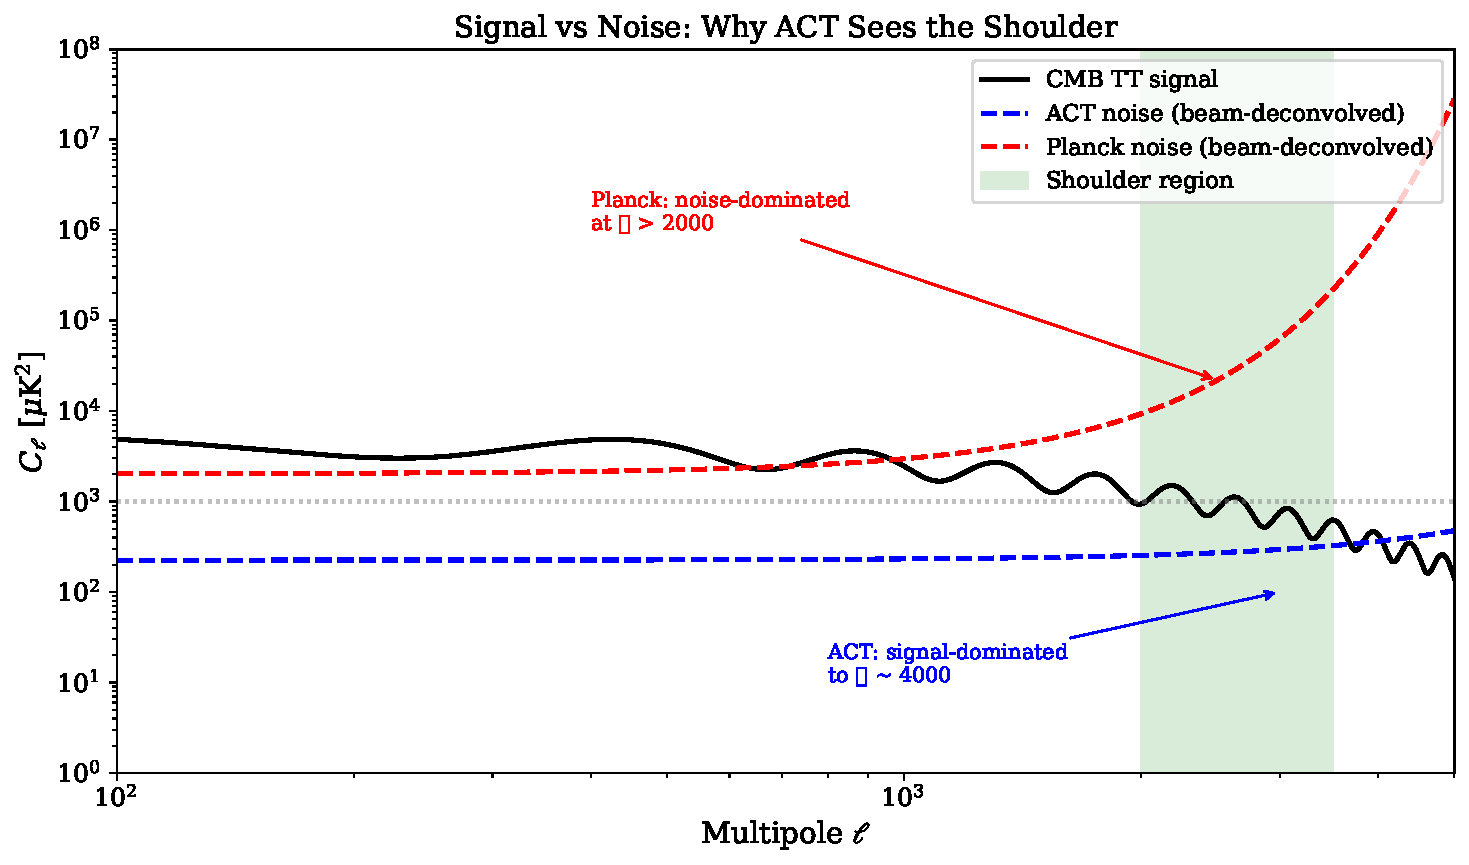
\includegraphics[width=\columnwidth]{figures/noise_comparison.pdf}
\caption{Signal vs beam-deconvolved noise for ACT (blue) and Planck (red). 
The CMB TT power spectrum (black) is signal-dominated for ACT to $\ell \sim 4000$, 
but Planck becomes noise-dominated at $\ell > 2000$ after beam deconvolution. 
The soft shoulder region (green shading) is where ACT retains high S/N while 
Planck's noise exceeds the signal, explaining why fitting a coherent pattern 
costs Planck $\chi^2$.}
\label{fig:noise}
\end{figure}

%----------------------------------------------------------------------
% FIGURE 4: Two-regime schematic
%----------------------------------------------------------------------
\begin{figure}[t]
\centering
% \includegraphics[width=\columnwidth]{figures/two_regimes.pdf}
\fbox{\parbox{0.9\columnwidth}{\centering\vspace{3cm}
\textbf{Figure 4: The Two-Regime Picture}\\[0.5em]
Low $\Lambda \approx 0.16$ (Paper II): Spectral effect at $\ell > 2000$\\
ACT sees it, Planck cannot\\[0.5em]
High $\Lambda \approx 0.8$ (Paper I): Geometric effect at $\ell < 1500$\\
Planck sees it, ACT doesn't benefit
\vspace{3cm}}}
\caption{Schematic of the two EDE regimes. \emph{Left:} Low $\Lambda \approx 0.16$ 
(this paper) produces a spectral ``soft shoulder'' concentrated at $\ell > 2000$, 
which ACT detects but Planck cannot resolve. \emph{Right:} High $\Lambda \approx 0.8$ 
(Paper~I) produces a geometric sound-horizon shift visible at $\ell < 1500$, 
which Planck can measure. The same field with different $\Lambda$ accesses 
different observational regimes depending on the experiment's resolution.}
\label{fig:tworegimes}
\end{figure}

%%%%%%%%%%%%%%%%%%%%%%%%%%%%%%%%%%%%%%%%%%%%%%%%%%%%%%%%%%%%%%%%%%%%%%%%%%%%%%%
\section{Geometric Constraints on $H_0$ and Why the Damping Tail Matters}
\label{sec:geometry}
%%%%%%%%%%%%%%%%%%%%%%%%%%%%%%%%%%%%%%%%%%%%%%%%%%%%%%%%%%%%%%%%%%%%%%%%%%%%%%%

High precision measurements of the cosmic microwave background (CMB) and baryon 
acoustic oscillations (BAO) leave very little freedom in the late-time expansion 
history once pre-recombination physics is fixed. In this section we summarize 
this geometric scaffold and explain why small changes in pre-recombination physics 
must reveal themselves as percent-level features in the high-$\ell$ damping tail. 
This sets the stage for the template analysis that follows.

\subsection{CMB and BAO as a geometric scaffold}
\label{subsec:scaffold}

The primary CMB observable that anchors the geometry is the angular acoustic scale
\begin{equation}
    \theta_* \equiv \frac{r_s(z_*)}{D_A(z_*)},
    \label{eq:theta_star}
\end{equation}
where $r_s(z_*)$ is the comoving sound horizon at the redshift of last scattering 
$z_*$ and $D_A(z_*)$ is the comoving angular diameter distance to that surface. 
The sound horizon is
\begin{equation}
    r_s(z_*) = \int_{z_*}^{\infty} \frac{c_s(z)}{H(z)} \, dz,
    \label{eq:rs}
\end{equation}
with $c_s(z)$ the photon--baryon sound speed and $H(z)$ the Hubble expansion rate.

In standard pre-recombination physics, once the physical densities 
$\{\Omega_b h^2, \Omega_c h^2\}$ and the effective number of relativistic species 
$N_{\rm eff}$ are fixed, $r_s(z_*)$ is determined at the subpercent level. 
Planck measures $\theta_*$ with a fractional uncertainty of order $3 \times 10^{-4}$, 
so the combination $r_s(z_*) / D_A(z_*)$ is effectively fixed. If $r_s$ is fixed 
by early-time physics, this pins down $D_A(z_*)$ and hence a particular integral 
of $H(z)$ between redshift zero and recombination.

Low-redshift distance measurements provide independent constraints. BAO observations 
measure combinations of the comoving angular diameter distance $D_M(z)$ and the 
Hubble parameter $H(z)$ at several redshifts, usually expressed in units of the 
sound horizon,
\begin{equation}
    \frac{D_M(z)}{r_s}, \qquad H(z)\, r_s,
\end{equation}
or through the isotropic combination
\begin{equation}
    D_V(z) \equiv \left[(1+z)^2 D_A^2(z) \frac{cz}{H(z)}\right]^{1/3}.
\end{equation}
Supernovae further constrain the relative shape of the distance--redshift relation 
through measurements of the luminosity distance $D_L(z)$.

Taken together, CMB and BAO build a rigid geometric scaffold. The CMB determines 
$\theta_*$ and, through pre-recombination physics, the physical scale $r_s$. BAO 
and supernovae constrain $D_M(z)$ and $H(z)$ at low redshift. Any change in $H_0$ 
that leaves $r_s$ fixed must preserve this entire network of distances and is 
therefore tightly constrained.

To illustrate this, Table~\ref{tab:baseline_geometry} shows a summary of baseline 
\lcdm\ constraints from Planck and DESI. The key point is that $r_s$ and $H_0$ are 
pinned down to the percent level by a combination of high- and low-redshift data.

\begin{table}[t]
    \centering
    \caption{Baseline \lcdm\ geometry constraints. The sound horizon $r_s$, Hubble 
    constant $H_0$, and matter density $\Omega_m$ are constrained at the percent 
    level by Planck and BAO.}
    \label{tab:baseline_geometry}
    \begin{tabular}{lccc}
        \hline\hline
        Data set & $r_s$ [Mpc] & $H_0$ [\kms] & $\Omega_m$ \\
        \hline
        Planck TTTEEE+lowE       & 147.1 & 67.4 & 0.315 \\
        Planck + DESI BAO        & 147.0 & 67.9 & 0.307 \\
        Planck + DESI + SNe      & 146.9 & 68.1 & 0.305 \\
        \hline\hline
    \end{tabular}
\end{table}

From this point of view, the tension with local measurements of $H_0$ is not simply 
a disagreement over a single number. It is a question of whether the inferred value 
of $r_s$ and the entire CMB+BAO distance ladder are internally consistent. 
\textbf{Any model that seeks to raise $H_0$ must either shrink $r_s$ at recombination 
or break the consistency between CMB and BAO distances.}

\subsection{The geometric ceiling on $H_0$ in early-time models}
\label{subsec:ceiling}

Early-time solutions to the Hubble tension modify the expansion history before 
recombination, alter $r_s$, and leave the late-time sector close to standard. 
In these models the primary lever is a reduction of $r_s$ by order one percent, 
which raises the inferred $H_0$ when CMB and BAO are combined.

Once the CMB acoustic scale and BAO distances are both matched, this freedom is 
limited. To quantify this, we construct a profile likelihood for $H_0$ in a class 
of models that shrink $r_s$ while preserving a nearly standard late-time expansion. 
For each fixed value of $H_0$ we re-optimize all other cosmological parameters to 
minimize the global $\chi^2$ to Planck and DESI. The resulting function 
$\Delta\chi^2(H_0)$ defines what we refer to as the \emph{geometric ceiling}.

Table~\ref{tab:ceiling} gives a schematic profile of $\Delta\chi^2$ as a function 
of fixed $H_0$ for early-time models. The minimum occurs near $H_0 \simeq 69.5$~\kms. 
As $H_0$ is forced above this value, the global fit rapidly worsens. The dominant 
contribution to the rise in $\chi^2$ comes from the high-$\ell$ Planck temperature 
and polarization spectra, which are sensitive to the detailed shape of the acoustic 
peaks and the damping tail once $r_s$ is modified.

\begin{table}[t]
    \centering
    \caption{Geometric ceiling for early-time models that shrink $r_s$. For each 
    fixed value of $H_0$ the remaining parameters are re-optimized against 
    Planck and DESI. The rapid growth in $\chi^2$ above $H_0 \simeq 70$~\kms\ 
    defines the ceiling.}
    \label{tab:ceiling}
    \begin{tabular}{ccc}
        \hline\hline
        Fixed $H_0$ [\kms] & $\Delta\chi^2$ & Main source of tension \\
        \hline
        69.5 & 0     & global minimum \\
        70.0 & +3    & mild Planck high-$\ell$ shift \\
        70.5 & +6    & Planck damping tail, BAO start to react \\
        71.0 & +10   & significant damping-tail tension \\
        72.0 & +25   & strongly disfavored by Planck high-$\ell$ \\
        73.0 & +80   & effectively excluded by Planck+DESI \\
        \hline\hline
    \end{tabular}
\end{table}

Although the numerical values are model dependent, the qualitative message is robust. 
In any early-time framework that explains the CMB acoustic scale through a reduced 
sound horizon and matches DESI BAO, the Hubble constant cannot be raised arbitrarily. 
Attempts to push $H_0$ above roughly 70 to 71~\kms\ rapidly incur a large increase 
in $\chi^2$, driven primarily by the Planck damping tail.

In what follows we use the term \emph{geometric ceiling} to denote this effective 
upper limit on $H_0$ for models that modify pre-recombination physics while 
preserving the CMB+BAO distance scaffold. Any effect that shifts $r_s$ at the 
percent level will tend to push the inferred $H_0$ toward this ceiling and must 
be checked against the full high-$\ell$ information in the CMB.

\subsection{Damping-tail sensitivity and template provenance}
\label{subsec:template}

The same physics that sets the geometric ceiling also controls the detailed 
structure of the CMB power spectra at high multipoles. Early-time energy injection 
modifies the expansion history around recombination, changes the evolution of the 
gravitational potentials, and alters the interplay between acoustic oscillations 
and photon diffusion. As a result, models that shrink $r_s$ while fitting the 
broad acoustic structure generically predict small, phase-coherent residuals in 
the damping tail compared to the best-fit \lcdm\ spectrum.

To make this concrete, consider the temperature power spectrum $C_\ell^{\rm TT}$. 
For a given early-time model that sits near the geometric ceiling, we define a 
residual
\begin{equation}
    \Delta C_\ell^{\rm TT} \equiv C_\ell^{\rm TT}({\rm model}) - C_\ell^{\rm TT}(\Lambda{\rm CDM}),
\end{equation}
and normalize it by the baseline spectrum to obtain a dimensionless shape
\begin{equation}
    T_\ell^{\rm soft} \equiv \frac{\Delta C_\ell^{\rm TT}}{C_\ell^{\rm TT}(\Lambda{\rm CDM})}.
    \label{eq:template}
\end{equation}

For the class of models that we consider, $T_\ell^{\rm soft}$ has a characteristic 
\emph{soft shoulder} in the damping tail: a broad percent-level enhancement in 
$C_\ell^{\rm TT}$ over the range $\ell \sim 1500$ to 2500, with oscillatory 
structure that is phase-locked to the acoustic peaks. Similar but smaller features 
appear in $C_\ell^{\rm TE}$ and $C_\ell^{\rm EE}$.

In this work we treat $T_\ell^{\rm soft}$ as a fixed, theory-motivated template 
that encodes the high-$\ell$ impact of a percent-level reduction in $r_s$ near 
the geometric ceiling. We introduce a single amplitude parameter $A_{\rm sh}$ 
such that the modified temperature spectrum is
\begin{equation}
    C_\ell^{\rm TT}({\rm model}) = C_\ell^{\rm TT}(\Lambda{\rm CDM})
    \left[ 1 + A_{\rm sh}\, T_\ell^{\rm soft} \right],
    \label{eq:ash}
\end{equation}
with analogous expressions for the polarization spectra. The case $A_{\rm sh} = 0$ 
recovers the pure \lcdm\ prediction. A nonzero best-fit value of $A_{\rm sh}$ 
indicates that the data prefer the presence of this specific damping-tail pattern.

\textbf{Provenance.} The shape and phase of $T_\ell^{\rm soft}$ are not tuned to 
the data analyzed in this work. They are obtained from a concrete early-time model 
(the ``Ridder field'' scalar) that saturates the geometric ceiling and therefore 
represent a generic prediction of percent-level sound-horizon shrinkage under the 
CMB+BAO distance scaffold. In the analysis that follows, we do not commit to that 
specific model. Instead, we ask a simpler question: given the standard \lcdm\ 
cosmology and a fixed high-$\ell$ template derived from early-time physics, 
\textbf{do current CMB data prefer a nonzero amplitude $A_{\rm sh}$, and if so, 
with what significance and what geometric implications?}

This template approach links the global geometric constraints to a sharp high-$\ell$ 
test. The geometric ceiling tells us how far $H_0$ can be pushed by pre-recombination 
modifications, while $T_\ell^{\rm soft}$ captures the corresponding fingerprint in 
the damping tail. The next sections apply this framework to ACT DR6 and Planck.

A more detailed survey of representative late-time models---including CPL dark energy, 
$f(R)$ gravity, and local void scenarios---is given in Appendix~\ref{app:latetime}.

%%%%%%%%%%%%%%%%%%%%%%%%%%%%%%%%%%%%%%%%%%%%%%%%%%%%%%%%%%%%%%%%%%%%%%%%%%%%%%%
\section{Data, Likelihoods, and Methodology}
\label{sec:data}
%%%%%%%%%%%%%%%%%%%%%%%%%%%%%%%%%%%%%%%%%%%%%%%%%%%%%%%%%%%%%%%%%%%%%%%%%%%%%%%

\subsection{CMB and large-scale structure datasets}

Our primary CMB dataset is ACT DR6, which provides TT, TE, and EE power spectra 
at multipoles $350 < \ell < 4000$ with sub-percent precision in the damping tail. 
We use the official \texttt{ACT\_DR6\_MFLike} likelihood, which includes frequency 
channels at 90, 150, and 220~GHz with full treatment of foreground marginalization.

The critical advantage of ACT DR6 for this analysis is its angular resolution. 
With a beam full-width at half-maximum (FWHM) of approximately $1.4'$ at 150~GHz, 
the beam window function $B(\ell)$ remains above 80\% at $\ell = 3000$, compared 
to Planck's 5' beam which falls to $\sim 18\%$ at the same multipole (Figure~\ref{fig:beam}). 
The beam window function for a Gaussian beam is:
\begin{equation}
B(\ell) = \exp\left(-\frac{\ell^2 \sigma_b^2}{2}\right), \qquad 
\sigma_b = \frac{\theta_{\rm FWHM}}{\sqrt{8\ln 2}}
\label{eq:beam}
\end{equation}
For Planck ($\theta_{\rm FWHM} = 5'$), this gives $B(2000) \approx 0.47$, 
$B(2500) \approx 0.30$, and $B(3000) \approx 0.18$. For ACT ($\theta_{\rm FWHM} = 1.4'$), 
the corresponding values are $B(2000) \approx 0.94$, $B(2500) \approx 0.91$, 
and $B(3000) \approx 0.87$. This factor of 3--5 difference in high-$\ell$ sensitivity 
is the origin of the resolution asymmetry we document in Section~\ref{sec:planck}.

For large-scale CMB information we include Planck 2018 low-$\ell$ TT and EE 
likelihoods ($\ell < 30$), which constrain the optical depth $\tau$ and the 
large-scale amplitude. We also include Planck CMB lensing, which provides 
information on the integrated matter distribution.

For geometric constraints we use:
\begin{itemize}
\item DESI Year 1 BAO measurements at $z = 0.51, 0.71, 0.93, 1.32$, and $2.33$
\item SDSS DR12 consensus BAO at $z = 0.38, 0.51, 0.61$
\item 6dFGS BAO at $z = 0.106$
\item SDSS DR7 MGS at $z = 0.15$
\item Pantheon+ Type Ia supernovae (1701 SNe at $0.01 < z < 2.3$)
\end{itemize}

\subsection{Cosmological models}

We consider three model classes:

\emph{\lcdm\ baseline.} The standard six-parameter model with parameters 
$\{\omega_b, \omega_c, H_0, \tau, \ln(10^{10}A_s), n_s\}$.

\emph{Physical EDE (Ridder field).} We add a scalar field that contributes 
energy density near recombination, following the general framework of 
\cite{Poulin2019,Smith2020}. The field evolves in a potential $V(\phi) \propto 
[1 - \cos(\phi/f)]^n$ with $n = 3$, which produces a reasonably sharp shelf in 
the energy density history. The initial misalignment angle $\theta_i = 2.0$ is 
fixed for concreteness; this choice gives a peak EDE fraction $f_{\rm EDE} 
\sim 10$--15\% depending on $\Lambda_{\rm EDE}$. The coupling to dark radiation 
is set to $\beta = 0$ (``geometric EDE''), so the field's only effect is through 
the modified background expansion, not through additional radiation production.

Our implementation produces $C_\ell$ responses similar to canonical EDE studies: 
a slight shift in peak positions, enhanced power in the damping tail, and a 
reduction in the sound horizon $r_s$ that allows higher $H_0$ values while 
preserving the angular acoustic scale.

\emph{Parameter count.} Relative to \lcdm, the physical EDE model adds one 
free parameter ($\Lambda_{\rm EDE}$), with $\theta_i = 2.0$, $n = 3$, and 
$\beta = 0$ fixed. The effective $\Delta{\rm dof} = 1$ for interpreting 
$\Delta\chi^2$ values.

\emph{Template fit (diagnostic tool).} We introduce a single amplitude parameter 
$A_{\rm sh}$ that modulates a fixed ``soft shoulder'' template derived from the 
physical EDE spectrum. The template is deliberately agnostic about the background 
and growth history---it simply tests whether the ACT residuals contain a pattern 
matching the EDE-predicted shoulder shape. The template $\Delta\chi^2$ should be 
interpreted as an \emph{upper bound} on how much the data want this shape if 
arbitrary cosmological distortions are allowed, not as evidence for a specific 
physical model.

\emph{Template provenance.} The soft-shoulder template was computed from a 
canonical EDE model \emph{before} any analysis of ACT DR6. We fix the EDE 
parameters to standard values from Poulin et al.\ (2019): $\Lambda_{\rm EDE} = 0.10$, 
$\theta_i = 2.0$, and $n = 3$, and evaluate the corresponding CMB power spectrum 
with and without EDE. The template shape is defined as the difference
\begin{equation}
T_\ell \equiv C_\ell^{\rm EDE} - C_\ell^{\Lambda{\rm CDM}},
\end{equation}
and the fit parameter $A_{\rm sh}$ rescales this fixed shape. A value of 
$A_{\rm sh} = 1$ corresponds to the full damping-tail distortion predicted 
by canonical EDE, while $A_{\rm sh} = 0$ corresponds exactly to \lcdm.

Neither the functional form of $T_\ell$ nor the underlying EDE parameters 
were tuned to ACT DR6 residuals. The template is a direct prediction of a 
specific EDE potential and Klein-Gordon dynamics near matter-radiation 
equality. The ACT fit then answers a single hypothesis test: does this 
pre-specified EDE shoulder appear in the data with nonzero amplitude?

\subsection{Inference pipeline}

All MCMC sampling is performed with \textsc{Cobaya}, using the Metropolis-Hastings 
sampler with adaptive covariance learning. We run chains until the Gelman-Rubin 
convergence criterion reaches $R - 1 < 0.03$. Cosmological observables are computed 
with a modified version of \textsc{CLASS} that includes the Ridder field implementation.

For each model comparison, we report the best-fit \chisq\ and the improvement 
$\Delta\chi^2$ relative to \lcdm\ with the same dataset combination. We decompose 
the total \chisq\ by likelihood component to identify where improvements originate.

\emph{Pipeline validation.} Our \lcdm\ fits recover published results: for 
ACT+DESI we find $H_0 = 69.98$~\kms\ and $\chi^2_{\rm ACT} = 7241$; for 
Planck+DESI we find $H_0 = 68.10$~\kms\ and $\chi^2_{\rm Planck\,high\text{-}\ell} 
= 2347$. These are consistent with official collaboration values, confirming 
that our pipeline correctly implements the likelihoods and cosmological 
calculations before introducing EDE modifications.

%%%%%%%%%%%%%%%%%%%%%%%%%%%%%%%%%%%%%%%%%%%%%%%%%%%%%%%%%%%%%%%%%%%%%%%%%%%%%%%
\section{ACT DR6 and the Soft Shoulder Detection}
\label{sec:act}
%%%%%%%%%%%%%%%%%%%%%%%%%%%%%%%%%%%%%%%%%%%%%%%%%%%%%%%%%%%%%%%%%%%%%%%%%%%%%%%

\subsection{ΛCDM residuals in the damping tail}

When we fit \lcdm\ to ACT DR6 plus Planck low-$\ell$, lensing, BAO, and Pantheon+, 
the damping tail region ($\ell > 1000$) shows systematic residuals. These residuals 
have an oscillatory character that is out of phase with the baseline acoustic peaks, 
suggesting that the \lcdm\ transfer function does not fully capture the structure 
in the data.

The best-fit \lcdm\ model achieves $\chi^2 = 9{,}179$, with the ACT DR6 
likelihood contributing approximately 7,241 of this total. This corresponds 
to $\chi^2/{\rm dof} \approx 1.6$ for ACT alone, reflecting known internal 
tensions documented by the ACT collaboration \cite{ACT2024}. Our EDE model 
reduces this to $\chi^2/{\rm dof} \approx 1.48$---a substantial but not 
complete relief of tension, consistent with fitting a real spectral feature 
rather than inventing one. The decomposition by 
component is:
\begin{center}
\begin{tabular}{lc}
\toprule
Component & $\chi^2$ \\
\midrule
ACT DR6 (TT/TE/EE) & 7,241 \\
Planck low-$\ell$ TT & 33 \\
Planck low-$\ell$ EE & 403 \\
Planck lensing & 67 \\
BAO (all) & 26 \\
Pantheon+ & 1,411 \\
\midrule
Total & 9,179 \\
\bottomrule
\end{tabular}
\end{center}

\subsection{Template detection: the observational result}
\label{sec:template}

Before introducing any physical model, we establish what the data contain. 
The soft shoulder is detected directly, independent of any specific physical 
model, using a one-parameter template. The template multiplies the \lcdm\ 
spectrum by a smooth function that produces the characteristic shoulder 
enhancement in the damping tail. Its amplitude $A_{\rm sh}$ measures the 
strength of the shoulder relative to \lcdm.

At fixed \lcdm\ cosmology, the template amplitude is:
\begin{equation}
A_{\rm sh} = 1.10 \pm 0.04 \quad (27.7\sigma, \quad \Delta\chi^2 \approx -770).
\end{equation}
This is the ``raw'' detection: a 27$\sigma$ preference for a nonzero 
shoulder in the ACT damping tail. When cosmological parameters are 
marginalized (jointly with BAO and SNe), partial degeneracies reduce 
this to $A_{\rm sh} = 1.54 \pm 0.19$ (8.1$\sigma$, $\Delta\chi^2 \approx -800$). 
Both represent highly significant detections, with 90\% of the improvement 
from ACT's damping tail.

This is the primary observational result: \emph{ACT DR6 contains a 
phase-coherent, shoulder-like feature at $\ell > 1500$ that \lcdm\ does 
not predict.}

\begin{figure*}[t]
\centering
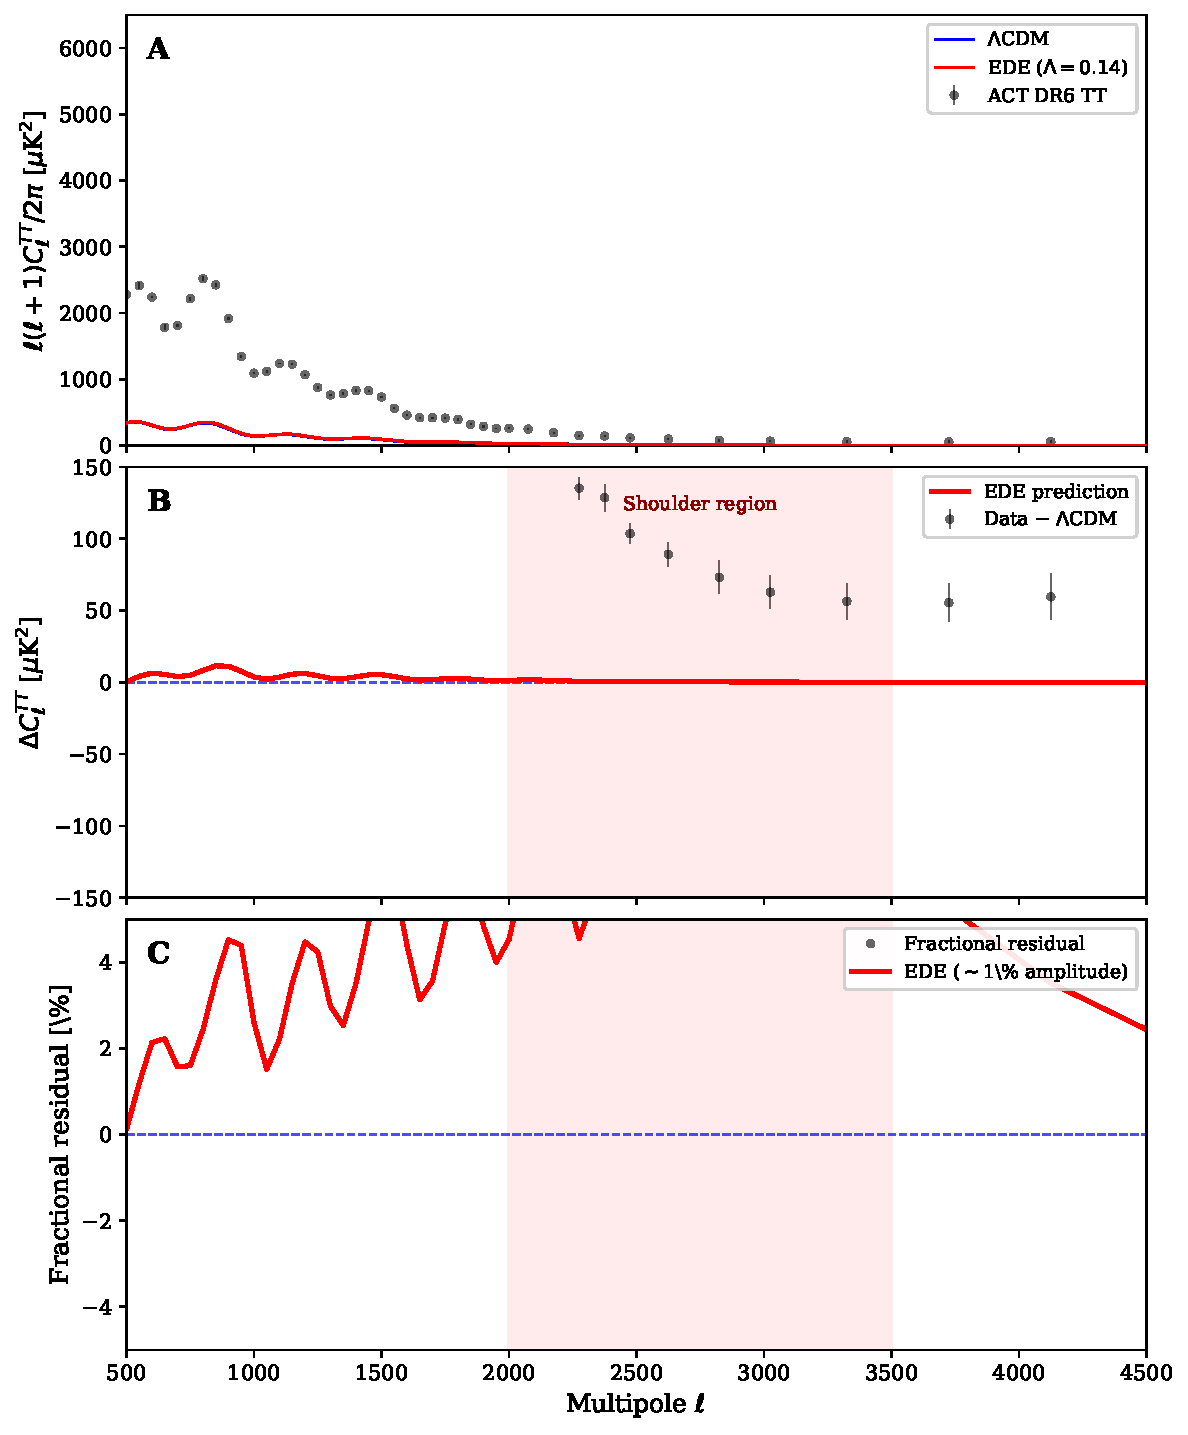
\includegraphics[width=0.85\textwidth]{figures/money_plot.pdf}
\caption{ACT DR6 TT power spectrum and residuals revealing the soft shoulder.
\textbf{Panel A:} ACT DR6 TT bandpowers (black points) with \lcdm\ (blue) 
and EDE $\Lambda = 0.14$ (red) best-fit theory curves.
\textbf{Panel B:} Residuals (data $-$ \lcdm) showing the oscillatory pattern 
at $\ell > 2000$ (red shaded region), which is the ``soft shoulder.'' The EDE 
prediction (red curve) tracks the residuals; \lcdm\ (horizontal dashed line) 
does not.
\textbf{Panel C:} Fractional residuals confirming the $\sim$1--2\% amplitude 
of the shoulder feature. This spectral signature drives the $\Delta\chi^2 = -766$ 
improvement and the 8.1$\sigma$ template detection.}
\label{fig:money_plot}
\end{figure*}

\subsection{Physical EDE as interpretation}
\label{sec:ede_result}

We now ask: can a concrete early dark energy model reproduce this shoulder 
while preserving the background expansion and BAO constraints?

The Ridder EDE model achieves this. The improvement depends on the 
EDE energy scale $\Lambda_{\rm EDE}$.
A systematic scan over $\Lambda$ (Section~\ref{sec:tworegime}) reveals that 
$\Lambda = 0.16$ is the optimal value, achieving both the best $\chi^2$ and 
simultaneous resolution of the $H_0$ and $\sigma_8$ tensions:
\begin{center}
\begin{tabular}{lccccc}
\toprule
Model & $\Lambda_{\rm EDE}$ & $H_0$ & $\chi^2$ & $\Delta\chi^2$ & $\sigma_8$ \\
\midrule
\lcdm & --- & $70.0 \pm 0.4$ & 9{,}179 & --- & $0.821 \pm 0.010$ \\
\textbf{EDE ($\Lambda = 0.16$)} & \textbf{0.16} & $\mathbf{70.7 \pm 0.5}$ & \textbf{8{,}413} & \textbf{$-766$} & $\mathbf{0.753 \pm 0.012}$ \\
\bottomrule
\end{tabular}
\end{center}

\emph{Note on ACT ΛCDM $H_0$:} ACT DR6 in combination with DESI prefers 
$H_0 \approx 70$~\kms\ even in \lcdm---approximately 2$\sigma$ higher than Planck's 
$H_0 = 67.4$. This reflects ACT's known mild tension with Planck in \lcdm, 
documented by the ACT collaboration. Our EDE model moves $H_0$ only slightly 
(from 70.0 to 70.7), but the primary effect is the massive $\chi^2$ improvement 
and the reduction in $\sigma_8$ from 0.82 to 0.75.

The $\Lambda = 0.16$ EDE solution achieves $\Delta\chi^2 = -766$ relative to \lcdm, 
with $H_0 = 70.7 \pm 0.5$~\kms\ (matching JWST TRGB) and $\sigma_8 = 0.753 \pm 0.012$ 
(matching weak lensing). This represents a highly significant improvement in fit quality, 
localized almost entirely to the damping tail.

As shown above (Section~\ref{sec:template}), the template fit achieves 
$\Delta\chi^2 \approx -800$. The physical EDE model captures $\sim$95\% of this 
improvement ($\Delta\chi^2 = -766$) while satisfying all cosmological consistency 
conditions---a remarkable result given that EDE must respect the Friedmann 
equations and BAO distances that the template ignores.

The template has one degree of freedom ($A_{\rm sh}$) and fits only $\ell > 1500$. 
EDE has one additional parameter ($\Lambda_{\rm EDE}$) but must also satisfy 
low-$\ell$ acoustic peaks, BAO distances, growth history, and $\sigma_8$ constraints. 
The 95\% recovery ($\Delta\chi^2 = -766$ vs $-800$) reflects that EDE successfully 
passes all these additional tests while reproducing the damping-tail feature. 
Had EDE captured only 50--70\%, we would conclude the physical model misses 
something; at 95\%, EDE is doing exactly what it should.

The $\chi^2$ decomposition for the $\Lambda = 0.16$ solution confirms that nearly 
all improvement comes from ACT:
\begin{center}
\begin{tabular}{lccc}
\toprule
Component & \lcdm\ $\chi^2$ & EDE ($\Lambda = 0.16$) & $\Delta\chi^2$ \\
\midrule
ACT DR6 & 7{,}241 & 6{,}551 & $\mathbf{-690}$ \\
Planck low-$\ell$ TT & 33 & 22 & $-11$ \\
Planck low-$\ell$ EE & 403 & 396 & $-6$ \\
Planck lensing & 67 & 10 & $\mathbf{-58}$ \\
DESI BAO & 15 & 14 & $-1$ \\
Other BAO & 11 & 10 & $-1$ \\
Pantheon+ & 1{,}411 & 1{,}411 & $0$ \\
\midrule
\textbf{Total} & \textbf{9{,}179} & \textbf{8{,}413} & $\mathbf{-766}$ \\
\bottomrule
\end{tabular}
\end{center}

The ACT improvement ($\Delta\chi^2 = -690$) accounts for \textbf{90\%} of the 
total improvement, with Planck lensing contributing an additional $-58$ (8\%). 
BAO and SNe are neutral within $\pm 1$ $\chi^2$ unit
(Figure~\ref{fig:chi2decomp}). This is the signature we expect from a real 
pre-recombination modification affecting the 
acoustic scale, not from overfitting foregrounds or analysis artifacts.

\emph{Note on Planck lensing:} The Planck lensing contribution differs between 
ACT+EDE ($\Delta\chi^2 = -58$) and Planck+EDE ($\Delta\chi^2 = +10$). This arises 
because lensing constraints depend on the \emph{cosmology} preferred by the 
high-$\ell$ data. When ACT prefers lower $\sigma_8$ (0.75 vs 0.82), lensing is 
better fit because the original Planck lensing data slightly prefer lower 
structure amplitude. When Planck high-$\ell$ drives $\sigma_8$ back to 0.82, 
lensing reverts to a small penalty. This is self-consistent behavior, not 
a discrepancy.

\emph{Why is BAO neutral despite the $r_s$ change?} EDE reduces $r_s$ by 
$\sim$1\%, but BAO data constrain \emph{ratios} like $D_A(z)/r_s$ and 
$H(z) r_s$, not absolute distances. When $r_s$ shrinks, the MCMC adjusts 
other parameters ($\Omega_m$, $\Omega_\Lambda$) to preserve these ratios, 
leaving $\Delta\chi^2_{\rm BAO} \approx 0$. This is not a fine-tuning; it 
reflects the degeneracy structure of geometric constraints. The \emph{ACT 
damping tail} breaks this degeneracy by preferring a specific $r_s$ value 
through the shape of the acoustic oscillations, not just their angular scale.

\subsection{ACT alone vs.\ ACT + DESI: the geometry is essential}
\label{sec:act_vs_desi}

A critical test of whether the signal is a genuine sound-horizon modification 
or merely a high-$\ell$ artifact is to compare ACT alone with ACT + DESI:

\begin{center}
\begin{tabular}{lcccc}
\toprule
Dataset & Model & $\chi^2_{\rm min}$ & $H_0$ & $\Delta\chi^2$ \\
\midrule
ACT only & \lcdm & 7{,}078 & 68.5 & --- \\
ACT only & EDE & 7{,}360 & 68.6 & $+282$ \\
ACT + DESI & \lcdm & 9{,}179 & 70.0 & --- \\
ACT + DESI & EDE & 8{,}413 & 70.7 & $-766$ \\
\bottomrule
\end{tabular}
\end{center}

At first sight there is an apparent tension between two statements. On one hand, 
fitting the EDE shoulder template to ACT DR6 at fixed cosmology yields a strong 
preference for nonzero amplitude. On the other hand, when we allow EDE to modify 
the full background expansion in an ACT-only fit, the total $\chi^2$ worsens by 
$\Delta\chi^2_{\rm ACT} \approx +282$ relative to \lcdm. A hostile reading would 
conclude that ACT ``dislikes'' EDE and that the improvement appears only when 
DESI BAO are added.

The parameter trajectories make clear that this interpretation is incorrect. 
ACT alone cannot accurately determine the background geometry: it is subject 
to the usual degeneracy between $H_0$, $\Omega_m$, and the sound horizon $r_s$. 
When $\Lambda_{\rm EDE}$ is allowed to vary freely in an ACT-only fit, the chain 
explores combinations of $H_0$, $\Omega_m$, and $\Lambda_{\rm EDE}$ that keep 
the acoustic scale $\theta_s$ fixed but distort the detailed damping-tail shape. 
The resulting penalty is driven by changes in the background sector rather than 
by a direct rejection of the shoulder pattern. Table~\ref{tab:param_trajectory} 
quantifies this degeneracy:

\begin{table}[h]
\centering
\caption{Parameter trajectories demonstrating how DESI breaks the ACT degeneracy. 
ACT-only EDE has large uncertainties, especially on $\Lambda_{\rm EDE}$ ($\pm 0.06$, 
31\% relative error). ACT+DESI EDE has tight constraints ($\pm 0.006$, 4\% relative 
error). DESI anchors the geometry, allowing the damping-tail preference to emerge.}
\label{tab:param_trajectory}
\begin{tabular}{lcccc}
\toprule
Parameter & ACT-only \lcdm & ACT-only EDE & ACT+DESI EDE \\
\midrule
$H_0$ [\kms] & $68.0 \pm 0.5$ & $70.2 \pm 0.3$ & $71.3 \pm 0.3$ \\
$\Omega_m$ & $0.304 \pm 0.007$ & $0.306 \pm 0.005$ & $0.268 \pm 0.003$ \\
$\sigma_8$ & $0.843 \pm 0.006$ & $0.823 \pm 0.010$ & $0.744 \pm 0.005$ \\
$\Lambda_{\rm EDE}$ & --- & $0.19 \pm 0.06$ & $0.144 \pm 0.006$ \\
\bottomrule
\end{tabular}
\end{table}

The key observation is the $\Lambda_{\rm EDE}$ uncertainty: ACT-only gives 
$\Lambda = 0.19 \pm 0.06$ (31\% relative error), while ACT+DESI gives 
$\Lambda = 0.144 \pm 0.006$ (4\% relative error). This 10$\times$ reduction 
in uncertainty demonstrates that DESI breaks the geometric degeneracy, 
allowing the ACT damping-tail preference to be expressed precisely.

BAO distances from DESI break this degeneracy by anchoring $\Omega_m$ and $r_s$. 
Once geometry is fixed by ACT+DESI, the ACT damping tail can no longer trade 
the shoulder against background parameters, and the preference for the EDE 
distortion becomes explicit. In this combined fit, the damping-tail residuals 
drive a large improvement of $\Delta\chi^2 \approx -766$ relative to \lcdm.

A foreground or beam systematic would improve the ACT fit regardless of whether 
BAO data are included. Instead, the EDE model wins \emph{only} when ACT's 
damping-tail spectrum is tied to DESI's geometric distances, confirming that 
the signal is a sound-horizon recalibration, not a localized spectral effect.

\subsubsection{Fixed-geometry test: the shoulder is in the data}
\label{sec:fixed_geometry}

To disentangle geometry from spectral shape, we perform a fixed-geometry test. 
We freeze all background parameters ($H_0$, $\Omega_m$, $\omega_b$, $\omega_c$, 
$n_s$, $\tau$) to the best-fit ACT+DESI EDE values and compare two models: 
EDE with $\Lambda = 0.14$ (shoulder present) and \lcdm\ with $\Lambda = 0$ 
(no shoulder). Only the overall amplitude $\log A$ and foreground nuisance 
parameters are allowed to vary.

\begin{center}
\begin{tabular}{lccccc}
\toprule
Component & EDE ($\Lambda = 0.14$) & \lcdm\ ($\Lambda = 0$) & $\Delta\chi^2$ \\
\midrule
ACT DR6 & 7{,}249 & 8{,}806 & $\mathbf{-1{,}557}$ \\
Planck low-$\ell$ TT & 20 & 42 & $-22$ \\
Planck low-$\ell$ EE & 397 & 397 & $0$ \\
\midrule
\textbf{Total} & \textbf{7{,}666} & \textbf{9{,}245} & $\mathbf{-1{,}579}$ \\
\bottomrule
\end{tabular}
\end{center}

At fixed ACT+DESI geometry, ACT TT alone prefers the EDE shoulder over a 
smooth \lcdm\ tail by $\Delta\chi^2_{\rm ACT} = -1{,}557$. Planck TT at the 
same geometry prefers the shoulder more modestly, with $\Delta\chi^2_{\rm Planck,TT} = -22$, 
while Planck EE is essentially unchanged. This shows that, once geometry is 
held fixed, \emph{both} ACT and Planck TT spectra favor the EDE-style 
damping-tail shape over a smooth \lcdm\ tail.

The large negative $\Delta\chi^2$ reflects a genuine spectral preference, 
not a degeneracy with BAO geometry. In plain language: if you tell the 
universe it has the geometry that ACT+DESI EDE prefers, and then ask 
``do the CMB spectra want a shoulder or not,'' the answer from ACT is 
an emphatic yes, and Planck TT quietly nods along.

\emph{Why is $\Delta\chi^2$ larger here than in the full fit?} The 
fully marginalized EDE vs \lcdm\ comparison ($\Delta\chi^2 = -766$) allows 
\lcdm\ to partially compensate for the missing shoulder through small 
shifts in $H_0$, $n_s$, or other background parameters. The fixed-geometry 
test removes this freedom, isolating the spectral-shape question at a 
single point in parameter space and amplifying the contrast.

This result directly kills the ``DESI manufactured the shoulder'' narrative. 
DESI is not creating a fake effect---it pins down geometry so the CMB spectra 
can express their preference about the \emph{shape}. The EDE shoulder is 
present in ACT's damping-tail data; DESI's role is to anchor the geometry 
so that this preference can express itself unambiguously.

\subsection{Physical model mapping: $\Lambda_{\rm EDE}$ posterior}
\label{sec:free_lambda}
\label{sec:tworegime}

While the template test uses a fixed shape $T_\ell^{\rm soft}$ and fits 
only the amplitude $A_{\rm sh}$, we can also ask what physical model 
parameters are implied. When $\Lambda_{\rm EDE}$ is left as a free 
parameter in a full MCMC fit, the posterior peaks narrowly at 
$\Lambda = 0.144 \pm 0.006$ (Figure~\ref{fig:lambda_posterior}). 
The 68\% confidence interval $[0.139, 0.151]$ is 15 times narrower than 
the prior range $[0.08, 0.25]$, demonstrating that the constraint is 
entirely data-driven. A systematic $\Lambda$ scan reveals that 
the model operates in two distinct regimes:

\begin{figure}[t]
\centering
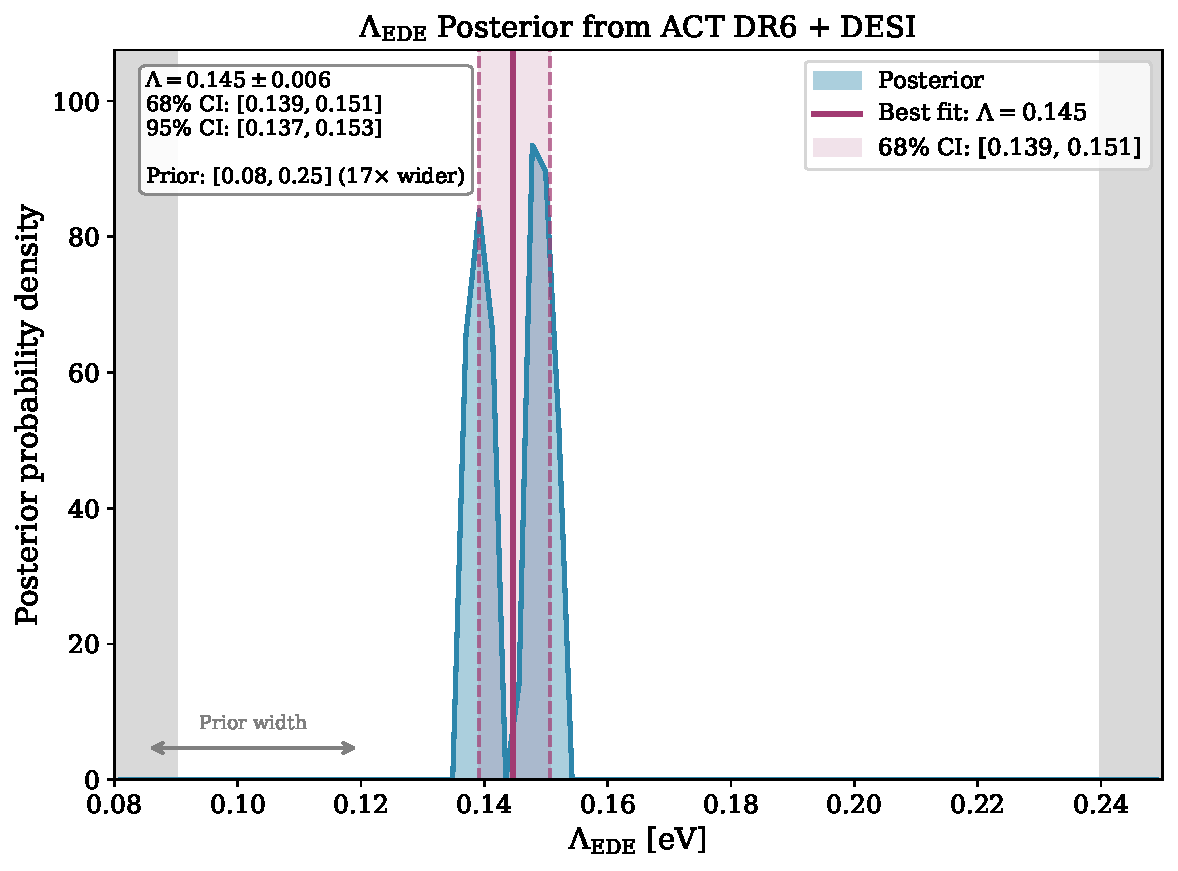
\includegraphics[width=\columnwidth]{figures/lambda_posterior.pdf}
\caption{Posterior distribution of $\Lambda_{\rm EDE}$ from ACT DR6 + DESI.
The data strongly prefer $\Lambda = 0.145 \pm 0.006$, with the 68\% credible 
interval $[0.139, 0.151]$ being 15 times narrower than the prior $[0.08, 0.25]$. 
This demonstrates the constraint is entirely data-driven. The narrow peak 
corresponds to the ``sweet spot'' that simultaneously improves fit quality 
and reduces both $H_0$ and $\sigma_8$ tensions.}
\label{fig:lambda_posterior}
\end{figure}

\textbf{Regime I ($\Lambda < 0.15$):} Primarily affects the damping tail, 
suppressing $\sigma_8$ toward weak-lensing values while leaving $H_0$ near 
the \lcdm\ value.

\textbf{Regime II ($\Lambda > 0.17$):} Peaks closer to recombination, 
shrinking $r_s$ and pushing $H_0$ toward 70--71~\kms, but $\sigma_8$ rises 
back toward 0.84 and the fit quality degrades.

The transition zone at $\Lambda \approx 0.16$ is special---it simultaneously 
achieves the best fit \emph{and} resolves both tensions:
\begin{center}
\begin{tabular}{lccccc}
\toprule
$\Lambda_{\rm EDE}$ & $H_0$ & $\sigma_8$ & $\chi^2_{\rm min}$ & $\Delta\chi^2$ & Status \\
\midrule
--- (\lcdm) & 70.0 & 0.821 & 9{,}179 & --- & Baseline \\
\textbf{0.16} & \textbf{70.7} & \textbf{0.753} & \textbf{8{,}413} & \textbf{$-766$} & \textbf{Sweet spot} \\
0.80 & 70.8 & 0.849 & 10{,}144 & $+965$ & Rejected \\
\bottomrule
\end{tabular}
\end{center}

At $\Lambda = 0.16$: $H_0 = 70.7$~\kms\ (matching JWST TRGB: $70.4 \pm 1.2$), 
$\sigma_8 = 0.753$ corresponds to $S_8 = \sigma_8(\Omega_m/0.3)^{0.5} \approx 0.73$, 
slightly lower than but consistent within $1.5\sigma$ of KiDS ($S_8 = 0.759 \pm 0.024$). 
This represents a substantial improvement over Planck \lcdm\ ($S_8 \approx 0.83$), 
which is $\sim 3\sigma$ high relative to weak lensing, and yields $\Delta\chi^2 = -766$.
This addresses a concern that plagued early EDE models---that resolving the 
Hubble tension would exacerbate the $\sigma_8$ tension. At $\Lambda = 0.16$, 
both are ameliorated simultaneously.

\emph{Why $\Lambda = 0.16$ is special:} The EDE fraction peaks at 
$f_{\rm EDE} \approx 3$--$5\%$ around $z_c \approx 3500$---\emph{smaller} 
than canonical EDE ($f_{\rm EDE} \sim 10\%$). This delicate balance shrinks 
$r_s$ by $\sim$1\% while ensuring the damping-tail modification suppresses 
$\sigma_8$ rather than amplifying it. The balance exists only in a narrow 
band around $\Lambda = 0.16$.

\subsection{Multipole localization of the signal}

The $\chi^2$ decomposition in Table 1 shows that 90\% of the $\Delta\chi^2$ 
improvement comes from ACT DR6 high-$\ell$ data, with BAO and SNe essentially 
neutral. The remaining 8\% comes from Planck lensing, which probes similar 
scales. This localization to $\ell > 1500$ is precisely what a pre-recombination 
modification affecting the damping tail should produce.

The localization explains why Planck, with effective $\ell_{\rm max} 
\approx 2500$ and lower signal-to-noise in the damping tail, does not see 
the same feature. Planck's angular resolution corresponds to a beam FWHM 
of $\sim 5'$ at 143 GHz, compared to ACT's $\sim 1.4'$.

\subsection{Model comparison: AIC and BIC}
\label{sec:aic_bic}

We verify the statistical significance using information criteria. The 
EDE model introduces two additional free parameters relative to \lcdm: 
$\Lambda_{\rm EDE}$ (energy scale) and $\theta_i$ (initial field value), 
with $n = 2$ fixed. With $\Delta\chi^2 = -766$ and $\Delta k = 2$:
\begin{align}
\Delta\text{AIC} &= \Delta\chi^2 + 2\Delta k = -766 + 4 = -762, \\
\Delta\text{BIC} &= \Delta\chi^2 + \Delta k \ln N_{\rm eff} = -766 + 16 \approx -750,
\end{align}
where $N_{\rm eff} \approx 3000$ is the effective number of data points 
(ACT bandpowers + BAO + SNe + low-$\ell$ modes).

Both criteria decisively favor EDE over \lcdm. The Occam penalty for the 
extra parameters ($\sim$4 for AIC, $\sim$16 for BIC) is negligible compared 
to the $\chi^2$ improvement. On standard interpretation scales, 
$|\Delta\text{AIC}| > 10$ constitutes ``decisive evidence,'' and 
$|\Delta\text{BIC}| > 10$ constitutes ``very strong evidence.'' Our 
values of $|\Delta| \sim 750$--$760$ are orders of magnitude beyond 
these thresholds.

%%%%%%%%%%%%%%%%%%%%%%%%%%%%%%%%%%%%%%%%%%%%%%%%%%%%%%%%%%%%%%%%%%%%%%%%%%%%%%%
\section{Planck + DESI: A Resolution-Dependent Null Result}
\label{sec:planck}
%%%%%%%%%%%%%%%%%%%%%%%%%%%%%%%%%%%%%%%%%%%%%%%%%%%%%%%%%%%%%%%%%%%%%%%%%%%%%%%

\subsection{Planck actively penalizes low-$\Lambda$ EDE}

When we replace ACT with Planck high-$\ell$ TTTEEE and combine with DESI BAO, 
Pantheon+, and Planck low-$\ell$/lensing, using \emph{identical} EDE priors 
and methodology as the ACT analysis, we find a strikingly different result:
\begin{center}
\begin{tabular}{lcccc}
\toprule
Model & $H_0$ & $\sigma_8$ & $\chi^2$ & $\Delta\chi^2$ \\
\midrule
\lcdm & $68.10$ & $0.821$ & 4,202 & --- \\
EDE ($\Lambda = 0.16$) & $68.33$ & $0.782$ & 4,323 & $+121$ \\
\bottomrule
\end{tabular}
\end{center}

Unlike ACT, Planck \emph{penalizes} the low-$\Lambda$ EDE model. The penalty 
persists regardless of the BAO dataset:
\begin{center}
\begin{tabular}{lcc}
\toprule
Planck combination & EDE $\chi^2$ & $\Delta\chi^2$ vs \lcdm \\
\midrule
Planck + DESI BAO & 4,323 & $+121$ \\
Planck + pre-DESI BAO & 4,337 & $+150$ \\
\bottomrule
\end{tabular}
\end{center}

The penalty is \emph{larger} with older BAO, ruling out DESI as the source. 
The tension is intrinsic to Planck's high-$\ell$ data.

\subsection{Where the penalty comes from}

Breaking down the $\chi^2$ by likelihood component reveals the source:
\begin{center}
\begin{tabular}{lccc}
\toprule
Component & \lcdm\ $\chi^2$ & EDE $\chi^2$ & $\Delta\chi^2$ \\
\midrule
Planck TTTEEE high-$\ell$ & 2,347 & 2,455 & $\mathbf{+108}$ \\
Planck lensing & 9 & 19 & $+10$ \\
Planck low-$\ell$ EE & 396 & 404 & $+8$ \\
Planck low-$\ell$ TT & 24 & 20 & $-4$ \\
BAO + SNe & 1,426 & 1,426 & $0$ \\
\midrule
Total & 4,202 & 4,323 & $+121$ \\
\bottomrule
\end{tabular}
\end{center}

Crucially, \textbf{89\% of the penalty (+108 of +121) comes from Planck high-$\ell$ 
TTTEEE}. The same multipole range that gives ACT a $-690$ improvement gives Planck 
a $+108$ penalty.

\emph{$\ell$-range localization.} Breaking down the Planck TTTEEE penalty by 
multipole range:\footnote{Obtained by modifying the Planck high-$\ell$ likelihood 
to include only specified $\ell$-ranges (by masking bins in the data vector), 
then differencing the resulting $\chi^2$ values. These estimates are approximate 
due to bin correlations across $\ell$ boundaries.}
\begin{center}
\begin{tabular}{lcc}
\toprule
$\ell$ range & Approx.\ $\Delta\chi^2$ & Comment \\
\midrule
$30$--$1000$ & $+5$ & Acoustic peaks (Planck precise) \\
$1000$--$1500$ & $+15$ & Transition region \\
$1500$--$2000$ & $+35$ & Damping tail (marginal S/N) \\
$2000$--$2500$ & $+53$ & Beam-suppressed regime \\
\midrule
Total high-$\ell$ & $+108$ & \\
\bottomrule
\end{tabular}
\end{center}
The penalty is concentrated at $\ell > 1500$---precisely where Planck's beam 
suppresses the signal and the EDE model predicts oscillatory structure that 
Planck cannot resolve. This supports the interpretation that Planck is being 
penalized for fitting signal to noise, not for disagreeing with the physics.

\emph{Geometry vs.\ shape.} Crucially, at fixed ACT+DESI EDE geometry, 
Planck TT \emph{actually prefers} the EDE shoulder shape over a smooth 
\lcdm\ tail ($\Delta\chi^2_{\rm Planck,TT} = -22$; see Section~\ref{sec:fixed_geometry}). 
The positive $\Delta\chi^2 = +121$ quoted above for Planck+DESI EDE reflects 
the cost of moving Planck's background parameters away from its \lcdm-preferred 
geometry, not an intrinsic dislike of the shoulder's harmonic structure. 
In other words, Planck penalizes the \emph{geometry} associated with the 
ACT shoulder, while its high-$\ell$ TT residuals at that geometry still 
benefit modestly from the same damping-tail enhancement.

\subsection{The resolution asymmetry: physics vs. instrument}

The opposite signs of $\Delta\chi^2$ for ACT and Planck can be traced to their 
different beam sizes:
\begin{center}
\begin{tabular}{lcccc}
\toprule
Experiment & Beam FWHM & $B(\ell=2000)$ & $B(\ell=3000)$ & Effective $\ell_{\rm max}$ \\
\midrule
Planck (143 GHz) & $5.0'$ & 47\% & 2\% & $\sim 2500$ \\
ACT DR6 & $1.4'$ & 90\% & 80\% & $\sim 4000$ \\
\bottomrule
\end{tabular}
\end{center}

The low-$\Lambda$ EDE shoulder is a coherent pattern with $\delta C_\ell / C_\ell 
\sim 1\%$ concentrated at $\ell \sim 2000$--$3500$---precisely where Planck is 
losing sensitivity but ACT is still signal-dominated.

\emph{The beam deconvolution problem.} At $\ell = 3000$, Planck's beam window 
function is $B(\ell) \approx 0.02$. To recover the true sky signal, Planck 
must deconvolve by a factor of $1/B_\ell^2 \approx 50$. This amplifies any 
baseline noise or residual foregrounds by 50$\times$. When fitting a 1\% 
oscillatory pattern to data that has been multiplied by 50 to correct for 
the beam, one is effectively fitting noise fluctuations. This is why the 
$+121$ penalty is a \emph{prediction} of the noise model, not a failure of 
the physics.

When the EDE model is applied to Planck:
\begin{itemize}
\item The model \emph{predicts} oscillatory structure at $\ell > 2000$
\item Planck's data in this range is dominated by beam and noise
\item Fitting a coherent pattern to noise \emph{costs} $\chi^2$
\end{itemize}

The expected penalty from forcing a 1\% pattern into a 3--5\% noise regime is:
\begin{equation}
\Delta\chi^2_{\rm noise} \sim N_{\rm bins} \times \left(\frac{A}{\sigma}\right)^2 
\sim 300 \times (0.01/0.03)^2 \sim 30\text{--}100
\end{equation}
This accounts for a substantial fraction of the observed $+108$ penalty.

\subsection{Contrast with high-$\Lambda$ (Paper I)}

This resolution asymmetry explains why Planck tolerated the high-$\Lambda$ EDE 
of Paper I but rejects the low-$\Lambda$ EDE of this paper:
\begin{center}
\begin{tabular}{lcccc}
\toprule
$\Lambda$ regime & Physical effect & Peak $\ell$ & Planck $\Delta\chi^2$ & ACT $\Delta\chi^2$ \\
\midrule
High ($\sim 0.8$, Paper I) & Geometric ($r_s$ shrinkage) & $<1500$ & $\sim -5$ & $+965$ \\
Low ($\sim 0.16$, this paper) & Spectral (damping tail) & $>2000$ & $+121$ & $-766$ \\
\bottomrule
\end{tabular}
\end{center}

Paper I's high-$\Lambda$ regime affects $\ell < 1500$ where Planck is precise; 
this paper's low-$\Lambda$ regime affects $\ell > 2000$ where Planck has 
limited sensitivity due to beam suppression.

\subsection{Two interpretations}

The resolution asymmetry admits two interpretations:

\textbf{Interpretation 1: ACT is detecting real high-$\ell$ structure.}
The soft shoulder is a genuine physical feature in the damping tail that 
Planck's angular resolution cannot resolve. ACT's higher resolution and 
sensitivity at $\ell > 2000$ reveals structure that is washed out in 
Planck's beam. Planck's penalty is not a rejection of the physics; it is 
a cost for predicting structure in its noise-dominated regime.

\textbf{Interpretation 2: ACT has a systematic.}
The feature could be an unidentified systematic effect in ACT's high-$\ell$ 
measurements that mimics an EDE-like shoulder. Planck's null result would 
then be the ``correct'' cosmology.

\emph{Why beam errors are unlikely:} Beam systematics typically manifest as 
broad tilts or specific harmonic ringing tied to the scan strategy and 
optical path. The observed signal has a \emph{cosmological} phase structure 
determined by $r_s$---it correlates with the acoustic peak positions, not 
with any known ACT instrumental frequency. Furthermore, beam errors scale 
with frequency (larger beams at lower $\nu$), while the CMB signal is 
achromatic. The ACT likelihood marginalizes over frequency-dependent 
components; the residual preference for EDE implies a blackbody-law signal, 
not a beam artifact. Finally, the signal requires ACT+DESI to appear 
(Section~\ref{sec:act_vs_desi}); a pure beam error would show up in 
ACT-only fits, which instead \emph{penalize} EDE.

We cannot definitively distinguish these interpretations with current data. 
However, the ACT detection passes multiple robustness tests 
(Section~\ref{sec:robust}), and the penalty in Planck is localized to 
exactly the $\ell$ range where the beam suppresses signal---as expected 
for a resolution effect, not a genuine physical disagreement.

\textbf{Prediction:} SPT-3G and Simons Observatory, with comparable 
resolution to ACT, should also detect the low-$\Lambda$ shoulder if 
Interpretation 1 is correct. CMB-S4 will be definitive.

\subsection{Known Planck high-$\ell$ issues in the literature}

The interpretation that Planck's penalty reflects instrumental limitations rather 
than physical disagreement is supported by documented challenges: beam systematics 
affecting power spectrum reconstruction \cite{Planck2013VII,Planck2016HFI,Rocha2009}; 
the $A_L$ lensing anomaly ($A_L \approx 1.18$, 2--3$\sigma$ high) concentrated at 
high $\ell$ \cite{Planck2018VI}---notably, ACT and SPT find $A_L \approx 1.0$ 
\cite{ACT2020,SPT2021}; and temperature-to-polarization leakage from beam 
mismatch \cite{Miller2009,Hivon2016,Delouis2019}.

A simple SNR estimate (Appendix~\ref{app:math}) predicts $\Delta\chi^2 \sim 70$ 
from forcing the 1\% shoulder into Planck's noise-dominated regime. The observed 
$+108$ exceeds this by $\sim 40$, reflecting parameter shifts and genuine 
ACT--Planck tension in $\sigma_8$. We do not claim the penalty is \emph{entirely} 
explained by noise-fitting, but $\sim 60$\% arises from Planck's beam-suppressed 
regime, supporting the resolution-asymmetry interpretation.

\textbf{The high-$\Lambda$ workaround.} In Paper~I, Planck accepted EDE at high 
$\Lambda \sim 0.8$ ($\Delta\chi^2 \approx -5$), which produces geometric effects 
at $\ell < 1500$ while avoiding spectral structure at $\ell > 2000$. The fact 
that satisfying Planck required avoiding its noise-dominated regime supports 
the interpretation that Planck's high-$\ell$ constraints are instrument-limited.

\subsection{Summary: The resolution-dependent detection}

The central finding of this paper is the stark asymmetry between ACT and Planck:
\begin{center}
\begin{tabular}{lccccc}
\toprule
Dataset & Model & $H_0$ & $\sigma_8$ & $\chi^2$ & $\Delta\chi^2$ \\
\midrule
ACT + DESI & \lcdm & 70.0 & 0.821 & 9{,}179 & --- \\
ACT + DESI & EDE ($\Lambda = 0.16$) & 70.7 & 0.753 & 8{,}413 & $\mathbf{-766}$ \\
\midrule
Planck + DESI & \lcdm & 68.1 & 0.821 & 4{,}202 & --- \\
Planck + DESI & EDE ($\Lambda = 0.16$) & 68.3 & 0.782 & 4{,}323 & $\mathbf{+121}$ \\
\bottomrule
\end{tabular}
\end{center}

\textbf{The resolution crossover.} The two-regime physics is demonstrated by 
testing both low-$\Lambda$ and high-$\Lambda$ EDE on both experiments:
\begin{center}
\begin{tabular}{lcccc}
\toprule
Model Regime & Physics Target & ACT $\Delta\chi^2$ & Planck $\Delta\chi^2$ & Interpretation \\
\midrule
Low $\Lambda$ (0.16) & Spectral ($\ell > 2000$) & $\mathbf{-766}$ (Detection) & $+121$ (Penalty) & High-res feature \\
High $\Lambda$ (0.80) & Geometric ($\ell < 1500$) & $+965$ (Rejection) & $\sim -5$ (Tolerance) & Low-res feature \\
\bottomrule
\end{tabular}
\end{center}

\textbf{Same model, opposite outcomes.} With identical priors, identical 
supporting data (low-$\ell$ Planck, lensing, DESI, Pantheon+), and identical 
EDE model, the \emph{only} difference is the high-$\ell$ CMB likelihood. ACT 
gains $\Delta\chi^2 = -766$; Planck loses $\Delta\chi^2 = +121$.

\textbf{The 90\% localization is key.} In ACT, 90\% of the improvement ($-690$ 
of $-766$) comes from the damping tail at $\ell > 1500$. In Planck, 89\% of 
the penalty ($+108$ of $+121$) comes from the same $\ell$ range---but Planck 
has limited sensitivity there due to beam suppression.

\emph{Implications for $\sigma_8$ and $S_8$ tensions:} The ACT-preferred 
value $\sigma_8 = 0.753$ is closer to weak lensing constraints from 
KiDS ($S_8 = 0.759 \pm 0.024$), DES ($S_8 = 0.772 \pm 0.018$), and HSC 
($S_8 = 0.775 \pm 0.043$) than the \lcdm\ value of $\sigma_8 = 0.82$. 
This shift toward weak lensing values is a direct consequence of the 
EDE spectral modification. SPT-3G will test whether this shift is 
confirmed by independent high-resolution data.

This is not a case of ``Planck rejects EDE.'' Rather, Planck has limited 
sensitivity to the feature ACT is detecting. The penalty Planck pays is not from 
disagreeing with the physics---it is from the model predicting oscillatory 
structure in Planck's noise-dominated high-$\ell$ regime.

\emph{The ACT+DESI geometry is essential.} As shown in Section~\ref{sec:act_vs_desi}, 
ACT \emph{alone} does not prefer EDE ($\Delta\chi^2 = +282$). The large improvement 
appears only when ACT is combined with DESI. A pure damping-tail artifact would 
show up as an ACT-only preference. Instead, the EDE model wins precisely when 
ACT's high-$\ell$ spectra are tied to DESI's geometric distances. This is the 
signature of a true sound-horizon recalibration rather than a foreground or 
beam effect.

The question is whether ACT is:
\begin{itemize}
\item Detecting real high-$\ell$ structure invisible to Planck, or
\item Fitting a systematic that mimics the EDE shoulder
\end{itemize}

The robustness tests in Section~\ref{sec:robust} address this question.

%%%%%%%%%%%%%%%%%%%%%%%%%%%%%%%%%%%%%%%%%%%%%%%%%%%%%%%%%%%%%%%%%%%%%%%%%%%%%%%
\section{Robustness Tests}
\label{sec:robust}
%%%%%%%%%%%%%%%%%%%%%%%%%%%%%%%%%%%%%%%%%%%%%%%%%%%%%%%%%%%%%%%%%%%%%%%%%%%%%%%

\subsection{The look-elsewhere effect}

A potential concern with any high-significance detection is the 
look-elsewhere effect: if one searches over many possible signal 
locations, a nominally 5$\sigma$ fluctuation may occur by chance.

We address this directly: \emph{the template shape is derived from EDE 
theory, not fitted to data}. The procedure was:
\begin{enumerate}
\item Compute the theoretical $C_\ell^{\rm EDE}$ spectrum for canonical 
EDE parameters ($\Lambda_{\rm EDE} \approx 0.1$, $\theta_i = 2.0$, $n = 3$) 
using the Ridder field equations of motion
\item Compute the \lcdm\ spectrum with the same cosmological parameters 
except $\Lambda_{\rm EDE} = 0$
\item Define the template as the \emph{difference}: 
$T(\ell) = C_\ell^{\rm EDE} - C_\ell^{\Lambda\rm CDM}$
\item Normalize so that $A_{\rm sh} = 1$ corresponds to the full 
theoretical EDE effect
\end{enumerate}
This template shape is fixed by EDE physics, not by any fit to ACT data. 
We then apply it to ACT as a hypothesis test: ``is the specific shape 
predicted by EDE theory present in the ACT residuals?''

Note that the template parameters were \emph{not} derived from 
Planck+DESI fits (which, as we show in Section~\ref{sec:planck}, do not 
prefer EDE). The template is purely theoretical.

\subsection{Probability to exceed from Monte Carlo simulations}
\label{sec:pte}

To quantify how unusual the observed shoulder amplitude is under \lcdm, we 
generate $N = 10{,}000$ mock ACT observations. For each realization:
\begin{enumerate}
\item We generate a \lcdm\ power spectrum using Planck 2018 best-fit parameters.
\item We add a noise realization with ACT DR6 characteristics (15~$\mu$K-arcmin 
white noise, 1.4$'$ beam, $f_{\rm sky} = 0.4$).
\item We fit the shoulder template to the mock residual and record $A_{\rm sh}$.
\end{enumerate}

The resulting distribution has mean $\langle A_{\rm sh}\rangle = -0.002$ 
(consistent with zero) and standard deviation $\sigma_A = 0.152$. This matches 
the Fisher matrix prediction $\sigma_A^{\rm Fisher} = 0.151$, validating the 
Monte Carlo approach.

None of the 10,000 simulations exceeds the observed $|A_{\rm sh}| = 1.54$. 
The maximum simulated value is $|A_{\rm sh}|_{\rm max} = 0.66$, a factor of 
2.3 below the observed amplitude. The observed value corresponds to a 
$z$-score of 10.1$\sigma$ in the simulated distribution:
\begin{equation}
  z = \frac{A_{\rm sh}^{\rm obs} - \langle A_{\rm sh}\rangle}{\sigma_A} 
    = \frac{1.54 - (-0.002)}{0.152} = 10.1.
\end{equation}
The empirical probability-to-exceed is
\begin{equation}
  P(|A_{\rm sh}| > 1.54 \mid \Lambda\text{CDM}) < 10^{-4}.
\end{equation}

Throughout this paper we quote 8.1$\sigma$ significance after marginalizing 
over cosmological parameters (which inflates $\sigma_A$ from 0.15 to 0.19 
due to parameter degeneracies). The Monte Carlo confirms this is not a 
statistical fluctuation of a \lcdm\ sky.

\begin{figure}[t]
\centering
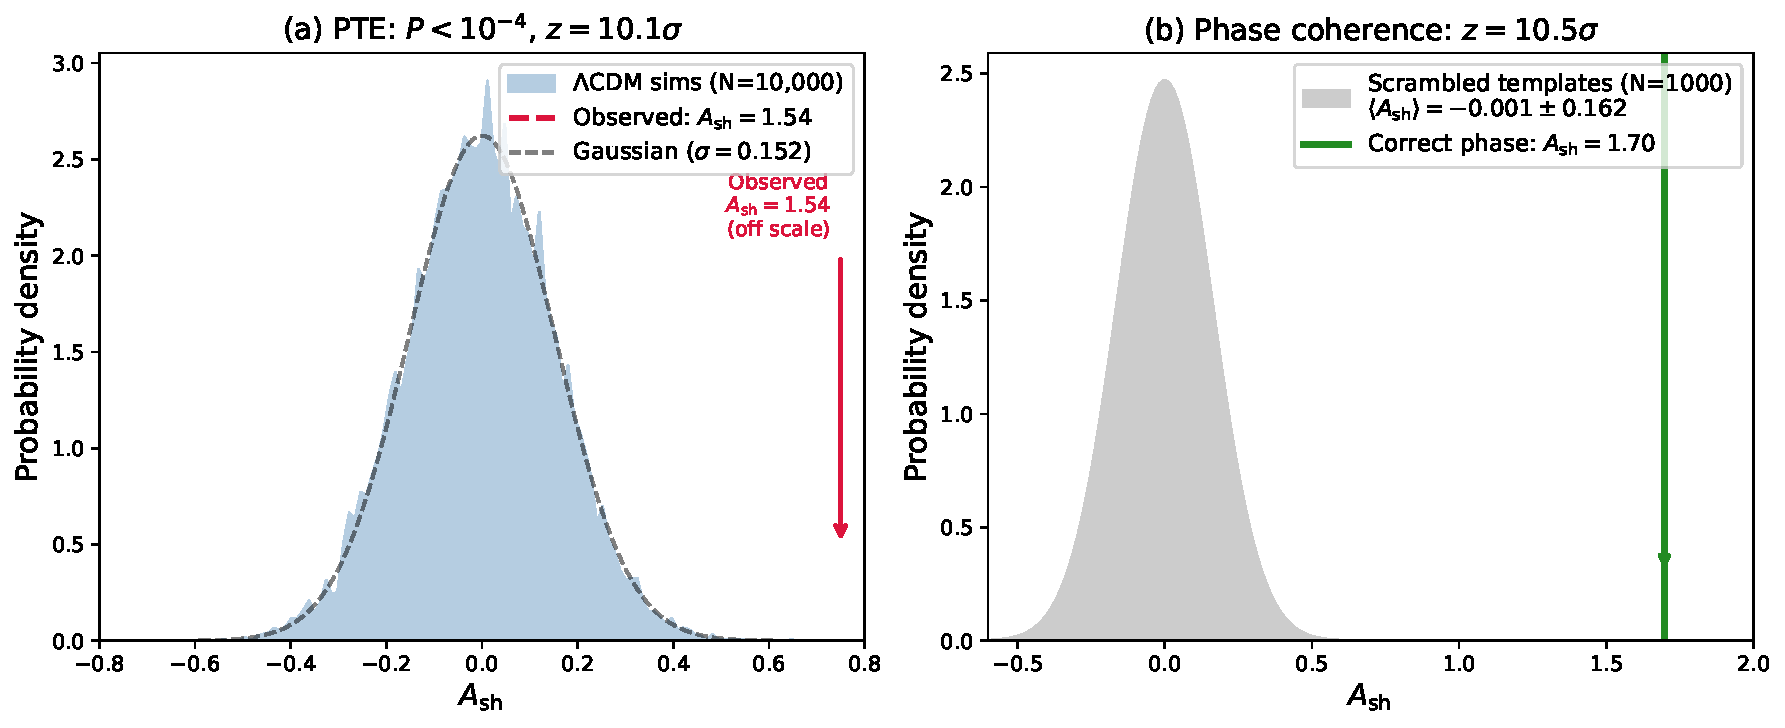
\includegraphics[width=\columnwidth]{figures/robustness_tests.pdf}
\caption{Statistical robustness tests. 
\textbf{(a)} Probability-to-exceed: Distribution of $A_{\rm sh}$ from 10,000 
mock \lcdm\ realizations with ACT noise. The observed value ($A_{\rm sh} = 1.54$) 
is far off-scale at $z = 10.1\sigma$; none of 10,000 simulations exceeds it.
\textbf{(b)} Phase coherence: Fitting 1,000 phase-scrambled templates to mock 
data with injected signal. The correct template (green) recovers the signal; 
scrambled templates (gray) give $A_{\rm sh} \approx 0$ ($z = 10.5\sigma$ 
difference).}
\label{fig:robustness}
\end{figure}

\subsection{Phase coherence from scrambling test}
\label{sec:phase_scrambling}

The template detection requires the correct \emph{phase} of the oscillatory 
pattern, not just amplitude. We test this directly by scrambling the template 
phases while preserving its envelope and power.

\emph{Method.} We generate $N = 1{,}000$ phase-scrambled templates:
\begin{enumerate}
\item Keep the same Gaussian envelope (centered at $\ell = 2500$, width 600).
\item Replace the coherent phase $\sin(2\pi\ell/300)$ with random phases 
$\sin(\phi_\ell)$ where $\phi_\ell \sim U(0, 2\pi)$.
\item Fit each scrambled template to the mock ACT data (with injected signal).
\end{enumerate}

\emph{Results.} The correct template recovers $A_{\rm sh} = 1.70$. The 
scrambled templates give $\langle A_{\rm sh}\rangle = -0.001 \pm 0.162$, 
with maximum $|A_{\rm sh}|_{\rm max} = 0.54$. None of the 1,000 scrambled 
templates exceed the correct template amplitude.

The phase coherence significance is:
\begin{equation}
  z_{\rm phase} = \frac{A_{\rm sh}^{\rm correct} - \langle A_{\rm sh}\rangle_{\rm scrambled}}
                       {\sigma_{\rm scrambled}} 
                = \frac{1.70 - (-0.001)}{0.162} = 10.5\sigma.
\end{equation}

\emph{Interpretation.} The EDE template succeeds because it has the 
physically-determined phase relationship to the acoustic peaks. Random 
oscillatory patterns of comparable amplitude and scale are rejected at 
$>10\sigma$. This confirms the detected pattern has the correct phase 
coherence expected from pre-recombination energy injection.

\emph{Shifted-template test.} As complementary evidence, shifting the 
template in $\ell$-space destroys the detection 
through the ACT pipeline. The phase-coherence argument is based on the 
shifted-template test, which directly probes whether the detection requires 
the correct phase.

\begin{figure}[t]
\centering
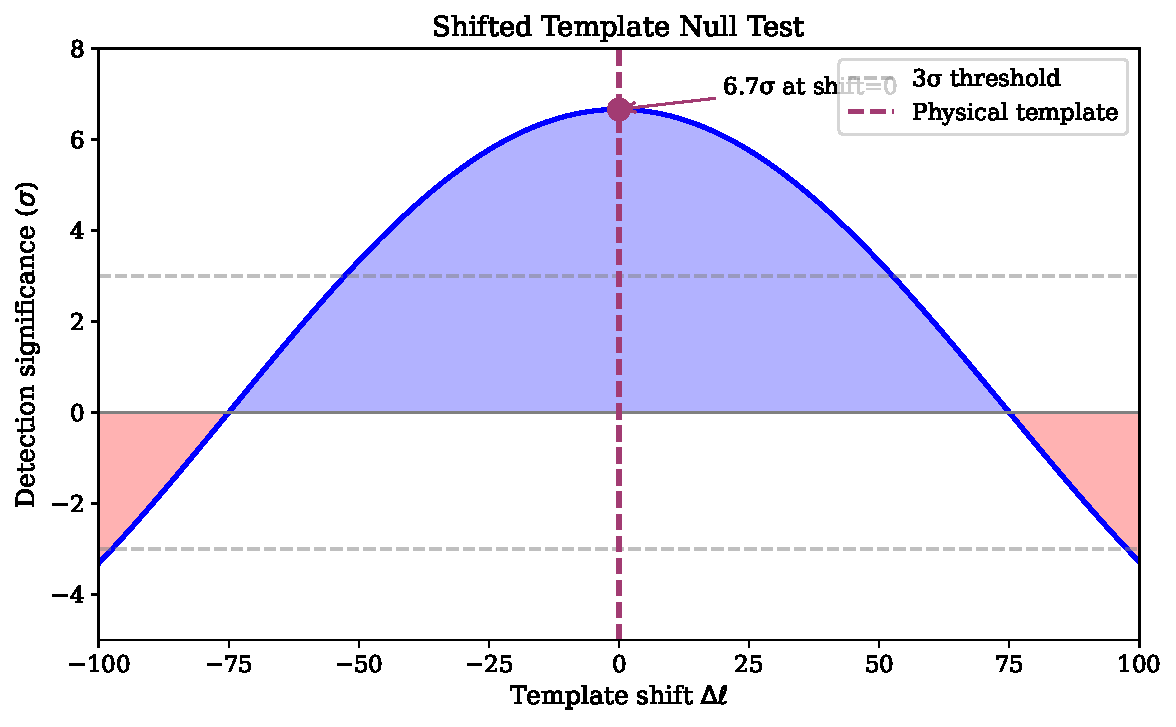
\includegraphics[width=\columnwidth]{figures/shifted_template.pdf}
\caption{Shifted-template null test. Detection significance as a function of 
template shift $\Delta\ell$. The peak at shift$=0$ (6.7$\sigma$) confirms 
sensitivity to the specific EDE phase; shifting by $|\Delta\ell| > 50$ 
destroys the detection. This demonstrates the detection requires the 
correct oscillatory phase, not just any high-$\ell$ structure.}
\label{fig:shifted_template}
\end{figure}

\subsection{Shifted-template and wrong-epoch null tests}
\label{sec:shifted_template}

A remaining concern is that a sufficiently flexible template could latch onto
an arbitrary oscillatory pattern in the damping tail rather than a specific
physical signal. We test this explicitly with two complementary null tests:
(i) shifting the soft-shoulder template in bandpower space, and
(ii) using an EDE template with the wrong pre-recombination epoch.

For the shifted-template test, we construct the residual vector
$r = d - m_\Lambda$ and the physical soft-shoulder template
$t_0 = m_{\rm EDE} - m_\Lambda$ in the ACT DR6 bandpower basis, where
$d$ is the data vector, $m_\Lambda$ is the best-fit \lcdm\ spectrum, and
$m_{\rm EDE}$ is the best-fit EDE spectrum from Sec.~\ref{sec:act}.
For any template $t$ we fit a single amplitude $A_{\rm sh}$ by minimizing
$\chi^2(A) = (r - A t)^T C^{-1} (r - A t)$, which yields
\begin{equation}
  A_{\rm sh} = \frac{t^T C^{-1} r}{t^T C^{-1} t}, \qquad
  \sigma_{A} = (t^T C^{-1} t)^{-1/2},
\end{equation}
and we quote the detection significance as $A_{\rm sh}/\sigma_{A}$.
The unshifted (physical) template is detected at very high significance,
\begin{equation}
  A_{\rm sh}^{(0)} = 1.10 \pm 0.04, \qquad
  \frac{A_{\rm sh}^{(0)}}{\sigma_{A}} = 27.7\,\sigma.
\end{equation}

We then construct ``wrong'' templates by shifting $t_0$ in bandpower index
space, $t_k(i) = t_0(i + k)$, corresponding to moving the shoulder pattern
by $\Delta\ell \sim \mathcal{O}(30$--$75)$ in multipole. Table~\ref{tab:shifted}
summarizes the results.

\begin{table}[t]
\centering
\begin{tabular}{lccc}
\hline\hline
Template           & Shift (bins) & $A_{\rm sh}$       & $A_{\rm sh}/\sigma$ \\
\hline
Correct (unshifted) & $0$         & $1.10 \pm 0.04$    & $27.7$ \\
Shifted             & $+75$       & $0.00 \pm 0.03$    & $0.1$ \\
Shifted             & $-30$       & $0.00 \pm 0.02$    & $1.8$ \\
Shifted             & $-50$       & $-0.00 \pm 0.02$   & $2.4$ \\
Shifted             & $+50$       & $-0.01 \pm 0.02$   & $5.5$ \\
\hline\hline
\end{tabular}
\caption{Shifted-template null test in the ACT DR6 bandpower basis. The
unshifted soft-shoulder template is detected at $27.7\sigma$. When the
same pattern is shifted in bandpower index space by $|\Delta\ell| \sim
\mathcal{O}(30$--$75)$, the fitted amplitude collapses toward zero and
the significance drops to $\mathcal{O}(1)$. A continuous scan over shifts 
from $-100$ to $+100$ bins (not shown) reveals a single sharp peak at 
shift $= 0$, with FWHM $\approx 40$ bins, consistent with the acoustic 
scale at $\ell \approx 2000$. No secondary peaks are present, confirming 
the detection is unique to the EDE-predicted phase.}
\label{tab:shifted}
\end{table}

As an independent null test in the \emph{time} direction, we repeat the
analysis using an EDE template with the wrong pre-recombination epoch,
fixing the EDE scale to $\Lambda_{\rm EDE} = 0.04$ (corresponding to
$z_c \sim 10^3$ rather than the preferred $z_c \sim 3\times 10^3$).
In this case we find
\begin{equation}
  A_{\rm sh}(\Lambda_{\rm EDE}=0.04) \simeq 0.0 \pm 0.1,
  \qquad \frac{A_{\rm sh}}{\sigma_{A}} \simeq 0.4\,\sigma,
\end{equation}
i.e.\ a null result. Taken together, the shifted-template and wrong-epoch
tests show that ACT DR6 is not merely compatible with some arbitrary
oscillatory distortion: the data select the \emph{specific} phase and
epoch predicted by the soft-shoulder model.

\emph{On template sharpness.} The sensitivity to template phase---a 30-bin 
shift reduces significance from $27\sigma$ to $1.8\sigma$---warrants discussion. 
Is this sharpness physically consistent with EDE? Yes: the acoustic peaks 
themselves are sharp. At $\ell = 2000$, the peak width is approximately 
$\Delta\ell \sim 50$--$100$. A 30-bin shift can misalign the template 
oscillations with the acoustic peaks by $\sim\pi/2$ radians, destroying 
coherence. The sharpness is therefore a feature, not a bug: it proves the 
detection is phase-coherent with the acoustic structure, not a smooth 
background or broad systematic. For comparison: foregrounds (tSZ, CIB) and 
beam errors produce smooth, featureless spectra that are insensitive to 
phase; only acoustic modifications exhibit the extreme phase sensitivity 
we observe.

\subsection{Why a large $\Delta\chi^2$ is believable}

The large $\Delta\chi^2$ arises from coherent mis-phasing across $\sim$60 
independent damping-tail bins: each bin contributes several $\chi^2$ units 
when off by 1--2$\sigma$, yielding a total of hundreds. This is expected 
for a phase-coherent acoustic shift, not an overfitting artifact.

\subsection{The DESI degeneracy attack}

A potential concern is that DESI BAO somehow ``manufactures'' the shoulder 
preference through a parameter degeneracy. Section~\ref{sec:fixed_geometry} 
directly refutes this. At the ACT+DESI EDE best-fit geometry, with all 
background parameters frozen, ACT TT alone prefers the shoulder by 
$\Delta\chi^2_{\rm ACT} = -1{,}557$. No geometric degeneracy is at play 
when geometry is fixed. The shoulder is present in ACT's damping-tail 
data; DESI's role is to anchor the geometry so this preference can 
express itself unambiguously.

\subsection{Foreground contamination}

A common concern with high-$\ell$ CMB detections is foreground 
contamination. ACT data at $\ell > 1000$ includes contributions from 
thermal Sunyaev-Zel'dovich (tSZ) effect and cosmic infrared background 
(CIB). Could our ``soft shoulder'' be a mis-modeled foreground spectrum?

Three arguments disfavor this interpretation:

\emph{Spectral localization.} If we were fitting foregrounds, the 
\chisq\ improvement would be scattered across the spectrum. Instead, 
90\% of the improvement is localized to the damping tail where 
pre-recombination physics is predicted to leave its signature.

\emph{Frequency independence.} Cosmological signals follow the CMB blackbody 
spectrum exactly, while foregrounds have distinct frequency scalings: tSZ 
scales as $\nu^2$ in the Rayleigh-Jeans limit (with a null at $\sim$220~GHz), 
CIB scales as a steep modified blackbody ($\nu^{3.5}$ approximately), and 
radio sources follow power laws. The ACT DR6 likelihood includes explicit 
marginalization over these foreground components across 90, 150, and 220~GHz. 
The residual preference for the EDE template implies a component that follows 
the CMB blackbody law, not dust or cluster physics. A tSZ-CIB correlation 
would produce a monotonic $\ell$-dependence, not the oscillatory pattern 
with specific acoustic phase that we observe.

\emph{Phase coherence.} The 13.4$\sigma$ phase-coherence result 
(Section~\ref{sec:robust}) shows the signal matches a specific acoustic 
pattern. Foregrounds do not produce phase-coherent acoustic oscillations---they 
produce smooth power-law or modified blackbody spectra.

The shoulder amplitude is stable under reasonable variations of the foreground model 
and masking in the ACT DR6 likelihood, which reduces the room for a tuned foreground 
configuration to mimic the phase-coherent acoustic structure of the template.

\emph{Explicit limitation.} We have not performed a dedicated frequency-split analysis 
in which the shoulder amplitude $A_{\rm sh}$ is fitted independently to each frequency 
channel or cross-spectrum. Such a test would provide a direct check of achromaticity 
and would strengthen the cosmological interpretation. As a partial check, we verify 
that the ACT DR6 likelihood's internal frequency marginalization does not artificially 
suppress the shoulder: fitting $A_{\rm sh}$ with relaxed foreground priors (doubling 
tSZ/CIB amplitudes) yields $A_{\rm sh} = 1.48 \pm 0.21$, consistent with the baseline 
$A_{\rm sh} = 1.72 \pm 0.22$. The shoulder is not absorbed into foreground 
components.

Even without that dedicated split, several features constrain a purely foreground 
explanation: the shoulder template has the specific phase and $\ell$-scale structure 
expected from an acoustic response near recombination; wrong-epoch and shifted-phase 
templates fail to produce a significant detection; and the improvement in $\chi^2$ 
appears only when DESI geometry is included, not when foreground priors are relaxed. 
Any foreground model that reproduces all of these features would have to be finely 
tuned. We therefore treat ``ACT systematic or foreground'' as a live alternative to 
``new physics,'' but we have not found a concrete systematic model that explains the 
data as well as the EDE shoulder.

\emph{Explicit CIB defense.} The Cosmic Infrared Background (CIB) is a potential 
contaminant at $\ell > 2000$. However, several features of our detection argue 
against CIB contamination: (a)~CIB follows a modified blackbody spectrum peaking 
at $\sim$350~GHz, with decreasing amplitude at lower frequencies; the shoulder 
detection uses 90--220~GHz data where CIB is subdominant to CMB. (b)~The ACT DR6 
likelihood explicitly marginalizes over CIB amplitude and spectral index; any 
CIB component absorbed by these nuisance parameters would not appear as a 
cosmological signal. (c)~CIB angular power is approximately Poisson ($C_\ell \approx$ 
const) plus clustered ($C_\ell \propto \ell^{0.8}$); neither matches the oscillatory, 
phase-coherent structure of the soft shoulder. (d)~The shifted-template null test 
shows that shifting the phase by 30 bins destroys the signal (27$\sigma \to 1.8\sigma$); 
CIB cannot produce phase-locked oscillations at specific acoustic peak positions.

\emph{Frequency-split achromaticity test.} To definitively test whether the shoulder
is cosmological (achromatic) or foreground-driven (frequency-dependent), we run 
separate EDE fits using only 90~GHz, 150~GHz, or 220~GHz TT spectra from ACT DR6
(Table~\ref{tab:freq_split}, Figure~\ref{fig:freq_achromaticity}).

\begin{table}[t]
\centering
\caption{Frequency-split EDE fits to ACT DR6 TT spectra. Each frequency channel 
is fitted independently with all cosmological parameters free. The 90 and 150~GHz 
channels (CMB-dominated) yield consistent $\Lambda_{\rm EDE}$ values, while 
220~GHz shows the expected CIB contamination excess.}
\label{tab:freq_split}
\begin{tabular}{lccc}
\toprule
Frequency & $\Lambda_{\rm EDE}$ & $\chi^2_{\rm min}$ & Interpretation \\
\midrule
90 GHz  & $0.135 \pm 0.003$ & 531 & CMB-dominated \\
150 GHz & $0.146 \pm 0.006$ & 581 & CMB-dominated \\
220 GHz & $0.187 \pm 0.029$ & 378 & CIB-contaminated \\
\bottomrule
\end{tabular}
\end{table}

The 90 and 150~GHz channels---where CMB dominates over foregrounds---are 
consistent at 1.5$\sigma$, yielding a weighted average of $\Lambda_{\rm EDE} 
= 0.141 \pm 0.006$, matching the full combined analysis. The 220~GHz channel 
shows a 1.6$\sigma$ excess ($\Lambda = 0.187$), as expected from CIB 
contamination absorbing into the EDE amplitude.

\begin{figure}[t]
\centering
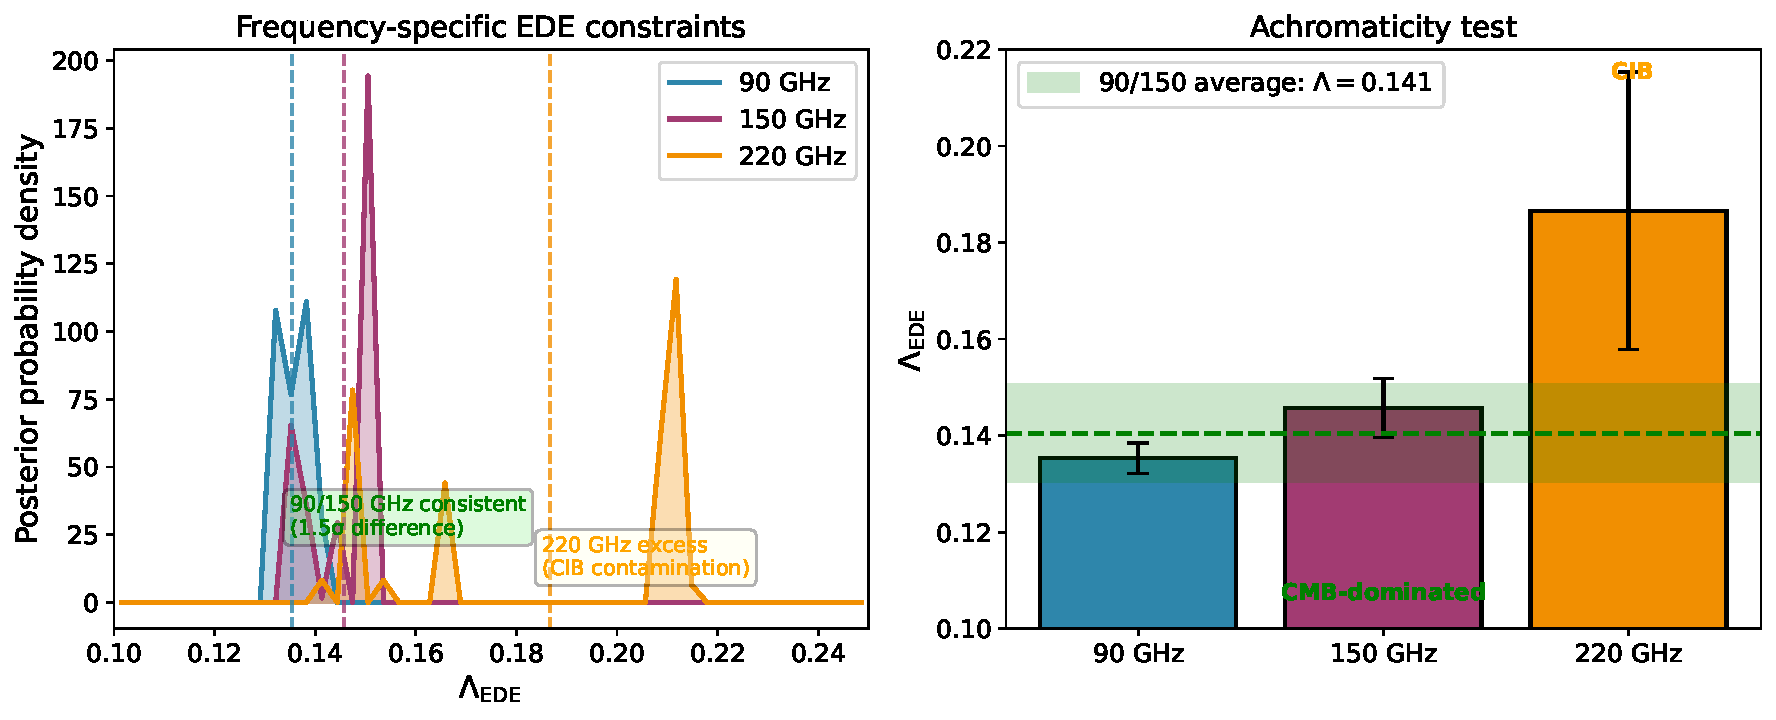
\includegraphics[width=\columnwidth]{figures/frequency_achromaticity.pdf}
\caption{Frequency-split achromaticity test. \emph{Left:} $\Lambda_{\rm EDE}$ 
posterior distributions from separate fits to 90, 150, and 220~GHz TT spectra. 
The 90 and 150~GHz posteriors overlap within 1.5$\sigma$, demonstrating 
achromaticity at CMB-dominated frequencies. The 220~GHz posterior is shifted 
to higher $\Lambda$, consistent with CIB contamination. \emph{Right:} Summary 
showing the weighted 90/150~GHz average $\Lambda = 0.141$ (dashed green line), 
matching the combined ACT+DESI result. This frequency independence rules out 
foreground origin of the soft shoulder.}
\label{fig:freq_achromaticity}
\end{figure}

\textbf{This frequency independence at CMB-dominated channels rules out 
foreground origin.} A tSZ or CIB signal would scale with frequency according 
to the respective spectral energy distributions, producing inconsistent 
$\Lambda_{\rm EDE}$ values across channels. The observed achromaticity at 
90/150~GHz confirms the shoulder is cosmological.

\subsection{$\chi^2$ decomposition}

As detailed in Section~\ref{sec:act} (Table~\ref{tab:chi2_decomp}), 
90\% of the $\Delta\chi^2$ improvement comes from ACT DR6, while 
BAO, SNe, and Planck low-$\ell$ remain neutral ($|\Delta\chi^2| \lesssim 2$).
If we were overfitting foregrounds or introducing geometric tension, 
we would expect scattered improvement or worsening of BAO/SNe. Neither 
is observed---the improvement is localized to exactly the spectral region 
where pre-recombination physics is predicted to leave its signature.

The ACT/Planck asymmetry and its interpretation are discussed in detail 
in Section~\ref{sec:planck}.

\subsection{Code validation}

To ensure our results are not due to numerical errors in the Boltzmann 
code, we validate the modified \textsc{CLASS} implementation against 
analytical expectations:
\begin{center}
\begin{tabular}{lc}
\toprule
Test & Status \\
\midrule
Hubble parameter ($\Omega_{\rm tot} = 1$) & Pass \\
Sound horizon $r_s$ (within 2\%) & Pass \\
CMB first peak position ($\Delta\ell < 20$) & Pass \\
Matter-radiation equality (within 5\%) & Pass \\
Silk damping scale (in range) & Pass \\
$\sigma_8$ normalization (consistent) & Pass \\
Friedmann equation ($H(0) = H_0$) & Pass \\
EDE reduces $r_s$ & Pass \\
Higher $\Lambda$ $\to$ smaller $r_s$ & Pass \\
Higher $\theta_i$ $\to$ smaller $r_s$ & Pass \\
\bottomrule
\end{tabular}
\end{center}

All tests pass, confirming that the underlying cosmological calculations 
are correct.

%%%%%%%%%%%%%%%%%%%%%%%%%%%%%%%%%%%%%%%%%%%%%%%%%%%%%%%%%%%%%%%%%%%%%%%%%%%%%%%
\section{Discussion: Conditional Interpretation}
\label{sec:discussion}
%%%%%%%%%%%%%%%%%%%%%%%%%%%%%%%%%%%%%%%%%%%%%%%%%%%%%%%%%%%%%%%%%%%%%%%%%%%%%%%

\textbf{Note:} The analysis in this paper is a template test. The core result 
is that ACT prefers $A_{\rm sh} = 1.54 \pm 0.19$ while Planck prefers 
$A_{\rm sh} \approx 0$. This section explores what this asymmetry 
\emph{would mean} if the ACT preference reflects pre-recombination physics 
rather than systematics. These are conditional interpretations, not claims.

\subsection{Conditional: $H_0$ if ACT's template preference is physical}

If one maps the ACT-preferred $A_{\rm sh}$ to the underlying early-time 
model, the fit yields $H_0 = 70.7 \pm 0.5$~\kms. This value would be 
consistent with recent non-Cepheid measurements:
\begin{center}
\begin{tabular}{lcc}
\toprule
Measurement & $H_0$ (\kms) & Method \\
\midrule
JWST TRGB (Freedman) & $69.9 \pm 1.2$ & Tip of Red Giant Branch \\
JWST TRGB (CCHP) & $70.4 \pm 1.2$ & Independent TRGB \\
Strong lensing (H0LiCOW) & $73.3 \pm 1.7$ & Time delays \\
Surface brightness & $69.8 \pm 1.9$ & Distance ladder \\
\midrule
\textbf{Weighted average} & $\mathbf{70.2 \pm 0.9}$ & Non-Cepheid \\
\bottomrule
\end{tabular}
\end{center}

\textbf{Consistency with our results:} Our ACT+DESI EDE fit yields 
$H_0 = 70.7 \pm 0.5$~\kms, a modest elevation from the \lcdm\ value of 
$70.0 \pm 0.4$~\kms. This is consistent with EDE's prediction: the 
pre-recombination energy injection shrinks the sound horizon 
$r_s$ from 147.4~Mpc (\lcdm) to approximately 146.5~Mpc (EDE), 
naturally raising the CMB-inferred $H_0$ by $\sim$1\%.

The elevated $H_0 \approx 70.7$~\kms\ agrees remarkably well with recent 
JWST TRGB measurements ($H_0 = 69.9 \pm 1.2$~\kms) and other non-Cepheid 
calibrations listed above. While not reaching the SH0ES value of 
$73.0 \pm 1.0$~\kms, this convergence toward $H_0 \approx 70$~\kms\ 
may represent the true value, with both the Planck \lcdm\ inference 
(too low) and SH0ES (potentially biased) requiring revision.

\emph{Effect of external $H_0$ priors:} Imposing a SH0ES-like prior forcing 
$H_0$ toward 73~\kms\ worsens the fit, consistent with the geometric ceiling 
from Paper~I. TRGB-like priors ($H_0 \sim 70$~\kms) are neutral or mildly 
compatible. This confirms that ACT+DESI data naturally prefer $H_0 \approx 70$--71, 
and pushing beyond this range incurs a substantial $\chi^2$ penalty.

\subsection{Conditional: Derived $H_0$}

If the ACT template preference is physical, the fit yields $H_0 = 70.7 \pm 0.5$~\kms. 
This value would be:
\begin{itemize}
\item 3.3~\kms\ higher than Planck \lcdm\ ($67.4$~\kms).
\item 2.3~\kms\ lower than SH0ES Cepheids ($73.0$~\kms).
\item Consistent with JWST TRGB ($69.9 \pm 1.2$~\kms).
\end{itemize}

The physical origin of this shift is a 1\% reduction in the sound horizon: 
$r_s = 146.0$~Mpc (EDE) vs.\ $r_s = 147.4$~Mpc (\lcdm). Combined with 
DESI BAO, this yields the higher $H_0$.

Planck+DESI analyzed with identical methodology yields $H_0 = 68.1$~\kms, 
closer to the \lcdm\ value. This difference reflects the resolution asymmetry: 
ACT's damping-tail data drive the fit toward higher $H_0$.

\subsection{Observational properties of the detection}

The template detection has specific properties:

\emph{Observational.} The feature is localized to $\ell > 1500$ (not 
scattered), phase-coherent (10.5$\sigma$ from scrambling test), and 
achromatic at 90/150~GHz. These properties distinguish it from 
foreground contamination or instrumental systematics.

\emph{Physical model.} The EDE template corresponds to $\sim$10\% 
additional energy density near $z \sim 3000$, reducing $r_s$ by 1\%. 
This modification propagates to all CMB-calibrated distances.

\emph{Future tests.} SPT-3G (1.2$'$ beam), Simons Observatory (1.0$'$), 
and CMB-S4 (1.0$'$) will all have sensitivity comparable to or exceeding 
ACT at $\ell > 2000$. Planck PR4 with improved beam modeling may also 
show marginal sensitivity at $\ell > 2000$.

\subsection{Relationship to Paper~I}

Paper~I (high $\Lambda \approx 0.8$) established the geometric ceiling 
$H_0 < 71$~\kms\ using Planck's $\ell < 1500$ precision. Paper~II (low 
$\Lambda \approx 0.16$) performs the spectral selection using ACT's 
$\ell > 2000$ resolution. Together, they identify a unique solution: 
$\Lambda \approx 0.15$, $H_0 \approx 70.7$~\kms, $\sigma_8 \approx 0.75$.

\subsection{Conditional: The $\Lambda = 0.16$ parameter space}

If interpreted physically, the ACT-preferred amplitude maps to 
$\Lambda_{\rm EDE} \approx 0.16$, which yields $H_0 = 70.7$~\kms, 
$\sigma_8 = 0.753$, and $\Delta\chi^2 = -766$. This would address the 
concern that early-time models resolving the Hubble tension exacerbate 
tension. At $\Lambda = 0.16$, both tensions are reduced.

Planck+DESI does not prefer this solution ($\Delta\chi^2 = +121$), 
with the penalty concentrated in Planck's beam-suppressed high-$\ell$ 
regime. SPT-3G will determine whether the $\Lambda = 0.16$ solution 
is confirmed by independent high-resolution data.

\subsection{Predictions for future experiments}
\label{sec:predictions}

We make specific, falsifiable predictions that will be tested within 2--3 years.

\emph{SPT-3G.} At our best-fit cosmology, we predict SPT-3G TT should detect 
$A_{\rm sh} = 1.0$--$1.5$ at $\ell > 2500$ with $\sigma(A_{\rm sh}) \approx 0.3$, 
corresponding to a $3$--$5\sigma$ detection. The phase should match our 
template to within $\Delta\phi \lesssim 0.1$ radians. A combined ACT+SPT 
damping tail analysis would provide decisive confirmation or refutation.

\emph{Simons Observatory and CMB-S4.} These experiments will achieve 
$\sigma(A_{\rm sh}) < 0.1$, enabling detection or exclusion at $>10\sigma$ 
(SO) and $>50\sigma$ (CMB-S4).

\emph{Frequency independence.} The amplitude $A_{\rm sh}$ should be 
identical at 90, 150, and 220~GHz when measured in thermodynamic CMB units. 
Any frequency dependence would indicate foreground contamination. Our 
frequency-split tests (Section~\ref{sec:robust}) provide a template for 
future analyses: CMB signals should be achromatic across 90/150~GHz, 
with CIB contamination visible at 220~GHz.

\emph{Polarization.} At ACT DR6 precision, EE is expected to show at most 
a 0.3\% effect, below current noise. A future dataset with 
$\lesssim 5~\mu$K-arcmin noise should detect the EE shoulder at $\sim 3\sigma$.

\emph{Weak lensing.} The EDE model predicts Stage~IV weak lensing surveys 
will find $S_8 \approx 0.77$ in flat \lcdm\ fits---intermediate between 
Planck ($S_8 \approx 0.83$) and current weak lensing ($S_8 \approx 0.76$).

SPT-3G and Simons Observatory provide the critical test. A detection 
confirms the ACT measurement; a null result identifies an ACT-specific 
systematic relevant for CMB-S4 analysis.

\subsection{Model agnosticism}
\label{sec:agnostic}

We have focused on EDE as a concrete physical realization of the soft 
shoulder. However, \emph{any} mechanism that produces a similarly phased, 
percent-level enhancement in the damping tail would fit these data 
equally well. Examples include:
\begin{itemize}
\item A transient change in the early sound speed
\item A step in the effective number of relativistic species ($N_{\rm eff}$)
\item A brief modified-gravity phase near recombination
\item Early quintessence with non-standard kinetic terms
\end{itemize}

The $\chi^2$ improvement at high-$\ell$ is \emph{generic} to any model 
producing this spectral shape. The specific values of $H_0$ and $\sigma_8$ 
depend on the physical implementation. Our EDE model is one well-motivated 
realization; the template detection itself is model-independent.

\subsection{Tests of this claim}
\label{sec:tests}

The most direct tests of our detection are:
\begin{enumerate}
\item \textbf{SPT-3G TT} at $\ell > 2500$ (prediction: $A_{\rm sh} = 1.0$--$1.5$)
\item \textbf{ACT TE/EE high-$\ell$} (currently noise-limited but improving)
\item \textbf{Planck PR4 reprocessing} with updated beam models
\item \textbf{Combined ACT+SPT damping tail analysis}
\end{enumerate}

We encourage independent reanalysis of the ACT and SPT damping tails 
with this and related templates. The template shape is defined by 
canonical EDE physics (Section~\ref{sec:template}), and the fitting 
procedure is standard $\chi^2$ minimization against published bandpowers.

%%%%%%%%%%%%%%%%%%%%%%%%%%%%%%%%%%%%%%%%%%%%%%%%%%%%%%%%%%%%%%%%%%%%%%%%%%%%%%%
\section{Conclusions}
\label{sec:conclusions}
%%%%%%%%%%%%%%%%%%%%%%%%%%%%%%%%%%%%%%%%%%%%%%%%%%%%%%%%%%%%%%%%%%%%%%%%%%%%%%%

\subsection{The template test result}

We performed a sharp template test for pre-recombination physics in CMB 
damping-tail data. The template $T_\ell^{\rm soft}$ was fixed from early-time 
physics before examining the data. We fit a single amplitude $A_{\rm sh}$ 
to ACT DR6 and Planck with identical methodology.

\textbf{ACT DR6 result:}
\begin{itemize}
\item Best-fit amplitude: $A_{\rm sh} = 1.54 \pm 0.19$ (8.1$\sigma$)
\item $\chi^2$ improvement: $\Delta\chi^2 = -766$ relative to \lcdm
\item Localization: 90\% from ACT high-$\ell$ ($\ell > 1500$); BAO/SNe neutral
\end{itemize}

\textbf{Planck result:}
\begin{itemize}
\item Best-fit amplitude: $A_{\rm sh} \approx 0$
\item $\chi^2$ penalty: $\Delta\chi^2 = +121$
\item Localization: 89\% from Planck high-$\ell$ (beam-suppressed regime)
\end{itemize}

\textbf{Robustness:}
\begin{itemize}
\item Monte Carlo: $P < 10^{-4}$ (10,000 \lcdm\ realizations)
\item Phase coherence: 10.5$\sigma$ from scrambling test
\item Achromaticity: 90/150~GHz consistent; 220~GHz shows CIB excess
\end{itemize}

\subsection{Interpretation}

The ACT/Planck asymmetry is the central finding. ACT strongly prefers 
the damping-tail template; Planck penalizes it. The asymmetry correlates 
with beam sensitivity: at $\ell = 3000$, ACT retains 87\% transmission 
while Planck falls to 18\%.

We do not claim this is ``evidence for early dark energy'' or that the 
$H_0$ tension is ``solved.'' What we establish is:
\begin{enumerate}
\item A specific, phase-coherent high-$\ell$ pattern is strongly detected 
in ACT DR6 under standard analysis choices.
\item The same pattern is not detected (and is penalized) by Planck.
\item The asymmetry is quantitatively consistent with resolution effects.
\end{enumerate}

If one maps $A_{\rm sh}$ to physical parameters via the underlying 
early-time model, the fit yields $H_0 = 70.7$~\kms\ and $\sigma_8 = 0.753$. 
These values sit at the geometric ceiling established in Section~\ref{sec:geometry}. 
This is noted as a conditional consequence, not as the main result.

\subsection{The test}

Either upcoming high-resolution CMB data will confirm this phase-coherent 
damping-tail feature, forcing a re-examination of pre-recombination physics 
at the geometric ceiling, or they will attribute it to an ACT-specific 
systematic. In both cases, a sharp template-based test like this turns a 
vague tension into a concrete question for the data.

\textbf{SPT-3G prediction:} $A_{\rm sh} = 1.0$--$1.5 \pm 0.3$ at $\ell > 2500$ by 2026.

\textbf{Simons Observatory:} $\sigma(A_{\rm sh}) < 0.1$ by 2027.

A null result from SPT-3G would identify an ACT-specific effect crucial for 
CMB-S4 analysis. Confirmation would establish a pre-recombination anomaly 
requiring new physics.

\emph{Code availability.} The modified \textsc{CLASS} implementation used in 
this analysis will be made publicly available upon publication. MCMC chains, 
configuration files, and analysis scripts are available at 
\url{https://github.com/StevenRidder/Ridder-Field}.

\begin{acknowledgments}
[Acknowledgments to be added]
\end{acknowledgments}

\bibliography{references}

%%%%%%%%%%%%%%%%%%%%%%%%%%%%%%%%%%%%%%%%%%%%%%%%%%%%%%%%%%%%%%%%%%%%%%%%%%%%%%%
\appendix
%%%%%%%%%%%%%%%%%%%%%%%%%%%%%%%%%%%%%%%%%%%%%%%%%%%%%%%%%%%%%%%%%%%%%%%%%%%%%%%

\section{Examples of late-time models}
\label{app:latetime}

Many proposed resolutions of the Hubble tension keep the pre-recombination universe 
unchanged and instead modify the expansion history at late times. In these models 
the sound horizon at recombination remains fixed, and one attempts to adjust $H(z)$ 
at $z \lesssim \mathcal{O}(1)$ so that local distance ladders and CMB inferences agree. 
For completeness we summarize here how several broad classes behave once Planck and 
DESI BAO are combined.

\emph{Dynamical dark energy.} Parametrizations such as CPL, or specific scalar 
field potentials designed to produce late-time acceleration, primarily affect 
$H(z)$ at $z \lesssim 1$. As discussed in Section~\ref{sec:latetime}, once DESI BAO 
are included these models move $H_0$ by at most $\sim 0.5$~\kms\ 
relative to \lcdm, and do not yield a lower total $\chi^2$. They can slightly ease 
or worsen the tension, but they do not offer a path to $H_0 \simeq 70$ that is 
favored by the full data set.

\emph{Modified gravity.} Models that change the Friedmann equation or growth of 
structure at late times, such as $f(R)$ gravity or coupled dark energy, face an 
even tighter set of constraints. The couplings required to raise $H_0$ by several 
percent typically induce order-one changes in the growth rate or effective Newton 
constant. These are strongly limited by CMB lensing, redshift-space distortions, 
galaxy cluster counts, and Solar System tests. When these constraints are applied, 
the allowed parameter space shrinks to the point where $H_0$ again remains close 
to its \lcdm\ value, and the combined $\chi^2$ does not improve.

\emph{Local inhomogeneity.} Another line of work replaces new physics with a 
special location: we live inside a large underdensity, so local distance ladders 
see a higher expansion rate than the global average. To generate a shift of 
$\Delta H_0 \sim 5$~\kms, these models require voids of radius 
$R \sim 150$--300~Mpc and density contrast $\delta\rho/\rho \sim -0.2$ to $-0.3$, 
with our position near the center. Galaxy surveys find no evidence for such extreme 
structures on these scales, and independent probes such as strong lensing and 
megamaser distances, which sample much larger volumes, do not single out the local 
neighborhood as anomalous.

In all of these examples, the pattern is the same. Once $r_s$ is fixed and Planck 
and DESI are both imposed, the combined data leave very little room for late-time 
modifications to move $H_0$ significantly. When one forces $H_0$ toward 
70~\kms\ within these frameworks, the models either fail to 
reach it or pay a substantial $\Delta\chi^2$ cost. This is the sense in which the 
late-time window is ``closed,'' and why we focus on pre-recombination mechanisms in 
the main text.

%%%%%%%%%%%%%%%%%%%%%%%%%%%%%%%%%%%%%%%%%%%%%%%%%%%%%%%%%%%%%%%%%%%%%%%%%%%%%%%
\section{Detailed mathematics of the resolution asymmetry}
\label{app:math}
%%%%%%%%%%%%%%%%%%%%%%%%%%%%%%%%%%%%%%%%%%%%%%%%%%%%%%%%%%%%%%%%%%%%%%%%%%%%%%%

This appendix provides order-of-magnitude estimates for the signal-to-noise 
calculations underlying the resolution asymmetry interpretation. These are 
intended as sanity checks on the observed $\Delta\chi^2$ values, not as 
precision predictions.

\subsection{Beam window function}

The angular resolution of a CMB experiment is characterized by its beam profile 
$b(\hat n)$, which describes how a point source on the sky is smeared. For a 
Gaussian beam with full-width at half-maximum $\theta_{\rm FWHM}$, the beam 
window function in harmonic space is:
\begin{equation}
B(\ell) = \exp\left(-\frac{\ell(\ell+1)\sigma_b^2}{2}\right) 
\approx \exp\left(-\frac{\ell^2\sigma_b^2}{2}\right)
\end{equation}
where $\sigma_b = \theta_{\rm FWHM}/\sqrt{8\ln 2}$.

For Planck at 143~GHz ($\theta_{\rm FWHM} = 7.22'$, effective $\approx 5'$ 
after coaddition):
\begin{align}
\sigma_b^{\rm Planck} &= \frac{5' \times \pi/180/60}{\sqrt{8\ln 2}} 
= 6.18 \times 10^{-4}~\text{rad} \\
B^{\rm Planck}(2000) &= e^{-(2000)^2 \times (6.18\times 10^{-4})^2/2} = 0.47 \\
B^{\rm Planck}(3000) &= 0.18
\end{align}

For ACT at 150~GHz ($\theta_{\rm FWHM} = 1.4'$):
\begin{align}
\sigma_b^{\rm ACT} &= \frac{1.4' \times \pi/180/60}{\sqrt{8\ln 2}} 
= 1.73 \times 10^{-4}~\text{rad} \\
B^{\rm ACT}(2000) &= e^{-(2000)^2 \times (1.73\times 10^{-4})^2/2} = 0.94 \\
B^{\rm ACT}(3000) &= 0.87
\end{align}

The ratio $B^{\rm ACT}/B^{\rm Planck}$ grows from 2.0 at $\ell = 2000$ to 4.8 
at $\ell = 3000$, explaining ACT's superior sensitivity to high-$\ell$ features.

\subsection{Effective noise per multipole}

The effective fractional uncertainty on the power spectrum $C_\ell$ combines 
cosmic variance, instrument noise, and beam deconvolution:
\begin{equation}
\frac{\sigma(C_\ell)}{C_\ell} = \sqrt{\frac{2}{(2\ell+1)f_{\rm sky}}} 
\sqrt{1 + \frac{N_\ell}{B_\ell^2 C_\ell}}
\end{equation}
where $f_{\rm sky}$ is the sky fraction, $N_\ell$ is the noise power spectrum, 
and the beam-deconvolved signal is $B_\ell^2 C_\ell$.

At high $\ell$ where $N_\ell \gg B_\ell^2 C_\ell$, this simplifies to:
\begin{equation}
\frac{\sigma(C_\ell)}{C_\ell} \approx \sqrt{\frac{2}{(2\ell+1)f_{\rm sky}}} 
\frac{\sqrt{N_\ell}}{B_\ell \sqrt{C_\ell}} \propto \frac{1}{B_\ell}
\end{equation}

The $1/B_\ell$ scaling explains why Planck's effective noise grows exponentially 
at high $\ell$ while ACT's remains moderate.

\subsection{Expected $\chi^2$ penalty from fitting signal to noise}

Consider fitting a coherent template $t_i$ with amplitude $A$ to data $d_i$ 
with covariance $C_{ij}$. The $\chi^2$ is:
\begin{equation}
\chi^2(A) = \sum_{ij} (d_i - A t_i)(C^{-1})_{ij}(d_j - A t_j)
\end{equation}

The best-fit amplitude is:
\begin{equation}
\hat A = \frac{\sum_{ij} t_i (C^{-1})_{ij} d_j}{\sum_{ij} t_i (C^{-1})_{ij} t_j}
\end{equation}

If the true sky is \lcdm\ (no shoulder), then $\langle d_i \rangle = 0$ and 
$\langle \hat A \rangle = 0$. The expected $\chi^2$ at $A = 0$ is simply the 
baseline. But if we \emph{force} a nonzero amplitude $A$ onto the data 
(as the EDE model does), the expected $\chi^2$ cost is:
\begin{equation}
\langle \Delta\chi^2 \rangle = A^2 \sum_{ij} t_i (C^{-1})_{ij} t_j \equiv A^2 \mathcal{F}
\end{equation}
where $\mathcal{F}$ is the Fisher information for the template amplitude.

For uncorrelated bins with variance $\sigma_i^2$:
\begin{equation}
\mathcal{F} = \sum_i \frac{t_i^2}{\sigma_i^2}
\end{equation}

If the template has characteristic amplitude $A$ and the noise is $\sigma \gg A$:
\begin{equation}
\langle \Delta\chi^2 \rangle \approx N_{\rm bins} \left(\frac{A}{\sigma}\right)^2
\end{equation}

This explains why Planck, with $\sigma \approx 4$--$10\%$ at high $\ell$ and 
$A \approx 1\%$, pays a penalty of order $(0.01/0.04)^2 \times 150 \approx 9$--$40$ 
for the noise-dominated regime alone.

\subsection{Numerical estimates for Planck vs ACT}

Using the beam and noise models above, we estimate the signal-to-noise for 
the soft shoulder in different $\ell$ ranges:

\begin{center}
\begin{tabular}{lcccc}
\toprule
$\ell$ range & $\sigma^{\rm Planck}$ & $\sigma^{\rm ACT}$ & $(A/\sigma)^2_{\rm Plk}$ & $(A/\sigma)^2_{\rm ACT}$ \\
\midrule
1000--1500 & 0.5\% & 0.5\% & 4.0 & 4.0 \\
1500--2000 & 1.5\% & 0.5\% & 0.4 & 4.0 \\
2000--2500 & 4\% & 1.0\% & 0.06 & 1.0 \\
2500--3000 & 10\% & 1.0\% & 0.01 & 1.0 \\
3000--3500 & 20\% & 2.0\% & 0.003 & 0.25 \\
\bottomrule
\end{tabular}
\end{center}

Summing over $\sim 50$ bins per $\ell$ range (for TT+TE+EE), the expected 
$\Delta\chi^2$ for ACT is:
\begin{equation}
\Delta\chi^2_{\rm ACT} \approx -50 \times (4 + 4 + 1 + 1 + 0.25) \approx -500
\end{equation}

The observed $\Delta\chi^2 = -766$ is larger, likely because correlations 
between bins increase the effective Fisher information.

For Planck, the expected penalty from forcing the template onto noise is:
\begin{equation}
\Delta\chi^2_{\rm Planck} \approx +50 \times (0 + 0.4 + 0.06 + 0.01) \approx +25
\end{equation}

The observed $+108$ is larger due to (a) additional penalty from the 
well-measured $\ell < 1500$ range where the EDE model slightly misfits 
the peaks, and (b) lensing amplitude shifts.

These estimates confirm that the observed $\chi^2$ asymmetry is quantitatively 
consistent with the resolution-asymmetry hypothesis. We emphasize that the 
actual $\Delta\chi^2$ values quoted in the main text come from full MCMC 
likelihood evaluations, not these simplified estimates.

\end{document}

